\documentclass[12pt]{article}

\usepackage{amsmath}
\usepackage{amssymb}
\usepackage{amsthm}
\usepackage{bm}
\usepackage{booktabs}
\usepackage{graphicx}
\usepackage{natbib}
\usepackage{geometry}
\usepackage{setspace}
\usepackage{hyperref}
\geometry{margin=1in}
\onehalfspacing

\newtheorem{theorem}{Theorem}
\newtheorem{lemma}{Lemma}
\newtheorem{proposition}{Proposition}
\newtheorem{assumption}{Assumption}
\newtheorem{corollary}{Corollary}
\theoremstyle{remark}
\newtheorem{remark}{Remark}

\title{\bf A Linear Programming Sensitivity Analysis for Parallel Trends\\
in Staggered Difference-in-Differences}
\author{Working draft}
\date{\today}

\begin{document}
\maketitle

\begin{abstract}
We develop a sensitivity analysis for the dynamic and overall average treatment effects on
the treated in staggered difference-in-differences designs. Both estimands are affine in
the conditional odds of adopting treatment at a given time rather than remaining untreated,
and letting those odds depend on the untreated trend encodes a violation of conditional
parallel trends. Replacing the odds by free variables constrained by the moment equations
the truth must satisfy, by a bound $\Lambda$ on how far selection may depart from what
covariates predict, and by a bound $\Lambda_\Delta$ on how fast that departure may change
across periods, yields worst-case bounds as the solution of a linear program, adapting the
estimating-equation approach of \citet{tang2025simple} from cross-sectional unmeasured
confounding. The bounds are sharp at the population level for a rich enough balance class,
converge at a near-root-$n$ rate, and deliver the whole event-study profile and the overall
effect from one feasible set. Pre-adoption periods calibrate the sensitivity parameters.
\end{abstract}

\section{Introduction}
\label{sec:intro}

Identification in staggered difference-in-differences (DiD) rests on a conditional
parallel trends assumption: among units not yet treated, the mean evolution of the
untreated potential outcome does not depend on the eventual adoption time, given
covariates. The assumption is untestable in exactly the periods where it is used, and it
fails whenever adoption timing is driven by the untreated trend itself. Applied practice
therefore needs a disciplined way of asking how far conclusions move when it is relaxed.

Two literatures bear on this problem, and they differ in what they restrict.

The first restricts the \emph{bias} directly. Writing the event-study coefficients as
$\beta = \tau + \delta$, with $\tau$ the causal effect and $\delta$ the violation of
parallel trends, \citet{rambachan2023honest} confine $\delta$ to a set $\Delta$ and report
the implied identified set. Their canonical choices restrict the \emph{shape} of $\delta$
over event time---bounded second differences, monotonicity, sign, or a bound on
post-treatment violations as a multiple of the largest pre-treatment one---and they supply
fixed-length and conditional confidence intervals with uniform validity over $\Delta$.
This is the standard approach in applied work, and it is well developed.

The second literature, built for unmeasured confounding in cross-sectional studies,
restricts the \emph{assignment mechanism} instead. \citet{rosenbaum1983assessing} bounds
the pairwise odds ratio of assignment, \citet{tan2006distributional} anchors the true
propensity score to a fitted one, and \citet{zhao2019sensitivity} and
\citet{dorn2023sharp} turn the resulting model into optimization over weights.
\citet{tang2025simple} go further within this line: rather than posit a parametric
propensity score and a departure from it, they treat the inverse propensity weights as
free variables constrained only by the estimating equations the truth satisfies, plus a
positivity bound, and obtain worst-case bounds from a linear program. Two features carry
over to our setting. The bounds hold under minimal assumptions, and they tighten
\emph{without} new assumptions as the class of estimating equations is enlarged.

This paper transplants the second approach to staggered DiD. That parallel trends is
itself a restriction on selection has been made precise by \citet{ghanem2022selection},
who characterise the forms of dependence between adoption timing and untreated potential
outcomes with which the assumption is compatible; we parametrise the departure from those
forms and bound its consequences. The untreated potential trend plays the role of the
potential outcome, selection on that trend the role of unmeasured confounding, and a
conditional odds the role of the inverse propensity weight. Our targets are the two
estimands applied work reports: the dynamic effect at each exposure duration, and the
overall effect.

Restricting the mechanism rather than the bias buys three things. The restriction is
conditional on covariates, so selection that varies across strata is handled natively. The
moment constraints force the reweighted comparison group to match the treated cohort in
covariates, so balance holds by construction. And the restriction is more primitive: a
bound on the odds implies a set of achievable biases whose size adapts to how dispersed
untreated trends are within strata (Proposition~\ref{prop:closed} gives the map
explicitly), whereas a set $\Delta$ is imposed on the bias irrespective of whether any
plausible selection could produce it. At the population level, under a balance class rich
enough to span the relevant covariate functions and relative to the periodwise sensitivity
model, the bounds are sharp (Theorem~\ref{prop:sharp}), and the whole event-study profile
together with the overall effect comes from a single constraint system.

We should be equally clear about what is not gained. Much of the power of
\citet{rambachan2023honest} comes from restricting the \emph{shape} of the violation
across event time, and our analogue---a bound $\Lambda_\Delta$ on how fast a unit's
departure may change between adjacent periods (Section~\ref{sec:range})---is a blunter
instrument, and our inference, which delivers consistency and a rate but not uniform
validity, is less developed than theirs. Section~\ref{sec:disc} takes up both points. The
two approaches are best read as complementary rather than one superseding the other.

Section~\ref{sec:setup} fixes notation and derives the odds representation on which the
method rests, Section~\ref{sec:sens} develops the sensitivity analysis,
Section~\ref{sec:sim} reports a simulation study, and Section~\ref{sec:disc} discusses how
the parameters should be chosen and what the method does not do.

\section{Setup and identification}
\label{sec:setup}

\subsection{Data, estimands and assumptions}

There are $T+1$ periods indexed $t = 0, 1, \ldots, T$, with $t = 0$ a baseline period in
which no unit is treated. Adoption is staggered and absorbing: a unit first treated in
period $g$ has treatment status $D_t = 0$ for $t < g$ and $D_t = 1$ for $t \ge g$. We
write $G = g$ for such a unit and $G = \infty$ for a unit never treated in the window, so
that $D_t = I(G \le t)$.

Let $Y_t(g)$ be the potential outcome in period $t$ under adoption at $g$, with
$Y_t(\infty)$ the never-treated potential outcome, and let $X$ be covariates measured at
baseline; Section~\ref{sec:disc} notes the extension to time-varying covariates. The
observed data are $n$ independent copies of $O = (G, X, Y_0, \ldots, Y_T)$. Write
$\Delta Y_t = Y_t - Y_{t-1}$ for the observed change and
$\Delta Y_t(\infty) = Y_t(\infty) - Y_{t-1}(\infty)$ for its never-treated counterpart.
Let $n_g = \#\{i : G_i = g\}$.

Our estimands are aggregates of cohort-by-period effects. For $1 \le g \le t \le T$,
the group-period ATT of \citet{callaway2021difference} is
\begin{equation}
\tau_{g,t} = E\{Y_t(g) - Y_t(\infty) \mid G = g\}.
\label{eq:cellatt}
\end{equation}
These cell effects are not themselves the object of applied interest; they are aggregated
across the triangular array $\{(g,t) : 1 \le g \le t \le T\}$. We target the two
aggregations that applied work reports. The \emph{dynamic} ATT at exposure duration
$s \in \{1, \ldots, T\}$ averages along a diagonal,
\begin{equation}
\tau^{\mathrm{dyn}}_s
= \frac{1}{p_s}\sum_{g=1}^{T-s+1} P(G{=}g)\,\tau_{g,\,g+s-1},
\qquad p_s = P(G \le T{-}s{+}1),
\label{eq:dyn}
\end{equation}
tracing the event-study profile, and the \emph{overall} ATT averages the whole triangle,
\begin{equation}
\tau = \frac{\sum_{g=1}^{T}\sum_{t=g}^{T} P(G{=}g)\,\tau_{g,t}}
            {\sum_{g=1}^{T}(T{-}g{+}1)P(G{=}g)}.
\label{eq:overall}
\end{equation}
Other aggregations---by cohort or by calendar period---are linear functionals of the same
cell effects and are handled identically; we do not treat them separately.

Nothing here restricts treatment effects to be homogeneous: the cell effects may differ
arbitrarily across cohorts and durations, and all the construction needs is that the target
be a linear aggregate of them with weights identified from the data.

The two targets are linked. Partitioning the triangle into its diagonals gives
\begin{equation}
\tau = \frac{\sum_{s=1}^{T} p_s\,\tau^{\mathrm{dyn}}_s}{\sum_{s=1}^{T} p_s},
\qquad
\sum_{s=1}^{T} p_s = \sum_{g=1}^{T}(T{-}g{+}1)P(G{=}g)
\label{eq:agg}
\end{equation}
(Lemma~\ref{lem:agg} in Appendix~\ref{app:proofs}, where all proofs are collected): the
overall effect is a weighted average of the event-study profile, with weights that decline
in $s$ because later durations are observed for fewer cohorts. Nothing is lost by studying
the profile, and the overall effect can be read off it. Its \emph{bounds} can be read off
too, but only in the absence of the cross-period restriction introduced in
Section~\ref{sec:range}; Section~\ref{sec:props} makes this precise. The population underlying
$\tau^{\mathrm{dyn}}_s$ shrinks as $s$ grows, so comparisons across durations mix effect
dynamics with cohort composition; restricting throughout to
$\{g : g \le T - s_{\max} + 1\}$ gives a balanced profile at the cost of sample size.

We maintain the following assumptions.

\begin{assumption}[Consistency]
\label{ass:cons}
$Y_t = Y_t(G)$ for every $t$.
\end{assumption}

\begin{assumption}[No anticipation]
\label{ass:na}
$Y_t(g) = Y_t(\infty)$ almost surely for every $t < g$.
\end{assumption}

\begin{assumption}[Conditional parallel trends]
\label{ass:pt}
$E\{\Delta Y_t(\infty) \mid X, G = g\} = E\{\Delta Y_t(\infty) \mid X, G = \infty\}$
for every $g$ and every $t \ge 1$.
\end{assumption}

\begin{assumption}[Positivity]
\label{ass:pos}
There is $\eta > 0$ with $P(G = g \mid X) > \eta$ almost surely for every
$g \in \{1, \ldots, T, \infty\}$.
\end{assumption}

Assumption~\ref{ass:pt} is the one we relax. Assumption~\ref{ass:na} is maintained
throughout: anticipation is a distinct failure mode and would need its own parameter.
Assumption~\ref{ass:pos} requires in particular a never-treated group, since the
comparison set at the last borrowing period is $\{G > T\}$; without one the cells $(g,T)$
are unidentified and the longest duration drops out.

\subsection{Identification and the odds representation}
\label{sec:odds}

We rewrite the standard identification formula so that the unknown propensity score enters
\emph{linearly}, through one scalar per cohort-period pair. The sensitivity analysis then
consists of letting those scalars vary.

Begin with identification itself. Fix $1 \le g \le r \le T$. By Assumption~\ref{ass:na}
the unit is untreated at $g-1$, so $Y_{g-1} = Y_{g-1}(\infty)$ for cohort $g$, and
\[
E(Y_r - Y_{g-1} \mid G{=}g) = E\{Y_r(g) - Y_{g-1}(\infty) \mid G{=}g\}.
\]
Subtracting $\tau_{g,r}$ leaves $E\{Y_r(\infty) - Y_{g-1}(\infty) \mid G{=}g\}$, which
telescopes into $\sum_{k=g}^{r} E\{\Delta Y_k(\infty) \mid G{=}g\}$. Each term is
unobserved, because cohort $g$ is treated in periods $k \ge g$. Assumption~\ref{ass:pt}
replaces it. The assumption is stated against the never-treated, whereas the comparison
sample below is the whole not-yet-treated set $\{G > k\}$; the two agree because
Assumption~\ref{ass:pt} holds for \emph{every} $g$, so every cohort untreated at $k$ has
the same conditional mean trend as the never-treated, and averaging over the composition
of $\{G > k\}$ preserves it:
\[
E\{\Delta Y_k(\infty) \mid X, G = g\} = E\{\Delta Y_k(\infty) \mid X, G > k\}
= E\{\Delta Y_k \mid X, G > k\},
\]
the last equality because units with $G > k$ are untreated at $k$ and $k-1$. Hence
\begin{equation}
\tau_{g,r} = E(Y_r - Y_{g-1} \mid G{=}g)
 - \sum_{k=g}^{r} E\big[\,\delta_k(X) \,\big|\, G{=}g\,\big],
\qquad \delta_k(X) = E\{\Delta Y_k \mid X,\, G > k\}.
\label{eq:identreg}
\end{equation}

Formula \eqref{eq:identreg} is a regression form: it requires the conditional mean
function $\delta_k$, then averages it over the covariate distribution of cohort $g$. That
outer average can instead be written as a weighted average over the units that are still
untreated, which produces the object we will make free. Define the conditional odds
\begin{equation}
a_{g,k}(X) = \frac{P(G = g \mid X)}{P(G > k \mid X)}, \qquad g \le k.
\label{eq:odds}
\end{equation}
Then for any integrable $\psi$,
\begin{equation}
E\{\psi(X) \mid G = g\}
 = \frac{1}{P(G{=}g)}\, E\big\{ I(G > k)\, a_{g,k}(X)\, \psi(X) \big\},
\label{eq:reweight}
\end{equation}
a reweighting identity that follows by conditioning on $X$
(Lemma~\ref{lem:reweight}). The interpretation is the familiar one for inverse
probability weighting. Units still
untreated at period $k$ are not representative of cohort $g$; weighting each by the odds
$a_{g,k}(X)$ that a unit with its covariates belongs to cohort $g$ rather than being still
untreated makes them so.

Applying \eqref{eq:reweight} with $\psi = \delta_k$, and then the tower property to absorb
$\delta_k$ back into $\Delta Y_k$, converts \eqref{eq:identreg} into the form we use.

\begin{proposition}[Odds representation]
\label{prop:oddsrep}
Under Assumptions~\ref{ass:cons}--\ref{ass:pos}, for $1 \le g \le r \le T$,
\begin{equation}
\tau_{g,r} = E(Y_r - Y_{g-1} \mid G{=}g)
 - \frac{1}{P(G{=}g)}\sum_{k=g}^{r} E\big\{ I(G>k)\, a_{g,k}(X)\, \Delta Y_k \big\}.
\label{eq:oddsrep}
\end{equation}
\end{proposition}

Two things about \eqref{eq:oddsrep} deserve emphasis, because the rest of the paper turns
on them. First, the outcome model $\delta_k$ has disappeared; the only unknown is the odds
$a_{g,k}$. Second, and decisively, $\tau_{g,r}$ is \emph{affine} in the collection
$\{a_{g,k}\}$, with coefficients that are functions of observed data. Optimizing over the
odds will therefore be a linear program rather than a general nonlinear one.

\subsection{Estimators for the two targets}
\label{sec:estimators}

Let $\widehat a_{g,k}$ denote a fitted value of \eqref{eq:odds}, obtained for instance by a
multinomial logistic regression of $G$ on $X$; \eqref{eq:odds} needs $P(G{=}g \mid X)$ for
each $g$ separately, so a proportional-odds fit would impose a restriction the
construction does not require. The sample analogue of \eqref{eq:oddsrep} is
\begin{equation}
\widehat\tau_{g,r}
= \frac{1}{n_g}\left[\ \sum_{i : G_i = g}(Y_{ir} - Y_{i,g-1})
 \ -\ \sum_{k=g}^{r}\ \sum_{i : G_i > k} \widehat a_{g,k}(X_i)\,\Delta Y_{ik}\ \right].
\label{eq:cellhat}
\end{equation}
The first sum is the observed long difference within cohort $g$; the second imputes the
counterfactual trend by reweighting the still-untreated units at each \emph{borrowing
period} $k = g, \ldots, r$. The two targets follow by aggregation.

\paragraph{Dynamic ATT.} Aggregating \eqref{eq:cellhat} along the diagonal
$r = g + s - 1$ with weights $\widehat P(G{=}g) = n_g/n$, the factors $n_g$ cancel. For
each borrowing period $k$, the cohorts whose horizon-$s$ cell needs it are
\begin{equation}
\mathcal{W}^{(s)}_k = \big\{\, g : \max(1,\, k{-}s{+}1) \le g \le \min(k,\, T{-}s{+}1) \,\big\},
\qquad
\Omega^{(s)}_k = \sum_{g \in \mathcal{W}^{(s)}_k} a_{g,k},
\label{eq:window}
\end{equation}
since cohort $g$ borrows period $k$ exactly when $g \le k \le g+s-1$. Hence
\begin{equation}
\widehat\tau^{\mathrm{dyn}}_s
= \frac{1}{N_s}\left[\ \sum_i I(G_i \le T{-}s{+}1)\,(Y_{i,G_i+s-1} - Y_{i,G_i-1})
 \ -\ \sum_{(i,k)\,:\,G_i > k} \Omega^{(s)}_k(X_i)\,\Delta Y_{ik}\ \right],
\label{eq:dynhat}
\end{equation}
with $N_s = \#\{i : G_i \le T{-}s{+}1\}$.

\paragraph{Overall ATT.} Aggregating \eqref{eq:cellhat} over the whole triangle instead,
the variable $a_{g,k}$ appears once for every endpoint $r$ with $k \le r \le T$, that is
$T-k+1$ times, and for every $g \le k$. Writing
\begin{equation}
\omega_k = \sum_{g \le k} a_{g,k},
\qquad
N_D = \#\{(i,t) : D_{it} = 1\} = \sum_i (T - G_i + 1)\,I(G_i \le T),
\label{eq:omega}
\end{equation}
the denominator $\sum_g (T{-}g{+}1)n_g/n$ becomes $N_D/n$ and
\begin{equation}
\widehat\tau
= \frac{1}{N_D}\left[\ \sum_i \sum_{r = G_i}^{T} (Y_{ir} - Y_{i,G_i-1})
 \ -\ \sum_{(i,k)\,:\,G_i > k} (T{-}k{+}1)\,\omega_k(X_i)\,\Delta Y_{ik}\ \right].
\label{eq:overallhat}
\end{equation}
Both normalizers are counts of treated cells and involve no propensity score, so both
estimators are affine in the odds, as promised.

\begin{remark}[Why the base period is $g-1$]
\label{rmk:base}
Any $l < g$ could serve as the base period in \eqref{eq:cellhat}, since under
Assumptions~\ref{ass:na}--\ref{ass:pt} the terms for $k = l+1, \ldots, g-1$ cancel in
population. The choice matters nonetheless. Anticipating the trend-dependent odds
\eqref{eq:tdodds} of Section~\ref{sec:model}, for $k < g$ the events satisfy
$\{G{=}g\} \subseteq \{G>k\}$, so
\begin{equation}
\alpha_{g,k}(x,\delta) = P\{G = g \mid X = x,\ \Delta Y_k(\infty) = \delta,\ G > k\},
\label{eq:preident}
\end{equation}
and every unit in the conditioning set has $\Delta Y_k$ observed: the quantity is point
identified. For $k \ge g$ the two events are disjoint and $\Delta Y_k(\infty)$ is
counterfactual for cohort $g$, so it is not. Taking $l = g-1$ confines the sensitivity
analysis to the unidentified part; an earlier base would add identified terms which, freed
as decision variables, widen the bounds for nothing. Section~\ref{sec:testable} uses
\eqref{eq:preident} in the opposite direction, to calibrate.
\end{remark}

\section{Sensitivity analysis}
\label{sec:sens}

\subsection{The sensitivity model}
\label{sec:model}

Assumption~\ref{ass:pt} fails when adoption timing depends on the untreated trend. We
encode exactly that by letting the odds \eqref{eq:odds} depend on it: for $g \le k$,
define the \emph{trend-dependent odds}
\begin{equation}
\alpha_{g,k}(X, \delta)
= \frac{P\{G = g \mid X,\ \Delta Y_k(\infty) = \delta\}}
       {P\{G > k \mid X,\ \Delta Y_k(\infty) = \delta\}}.
\label{eq:tdodds}
\end{equation}
We assume throughout the \emph{finiteness condition} that
$P\{G > k \mid X, \Delta Y_k(\infty)\} > 0$ almost surely on the support of
$(X, \Delta Y_k(\infty))$ given $G = g$, so that $\alpha_{g,k}$ is finite.
Assumption~\ref{ass:pos} does not imply this, since conditioning on the trend can empty
the comparison set where covariates alone do not; any range restriction of
Section~\ref{sec:range} implies it. If $\alpha_{g,k}$ does not depend on $\delta$ it equals
$a_{g,k}(X)$, and if this holds for every $g \le k$ then each cohort $g \le k$ is
conditionally independent of the period-$k$ untreated trend given $X$. Dependence on
$\delta$ \emph{is} selection on the untreated trend. The following lemma, elementary but
doing all the work, is the trend-dependent counterpart of \eqref{eq:reweight}.

\begin{lemma}[Restoration]
\label{lem:restore}
For any $\psi$ with $E\{I(G{=}g)\,|\psi(X, \Delta Y_k(\infty))|\} < \infty$,
\begin{equation}
E\big\{ I(G{>}k)\, \alpha_{g,k}\big(X, \Delta Y_k(\infty)\big)\,
 \psi\big(X, \Delta Y_k(\infty)\big)\big\}
= E\big\{ I(G{=}g)\, \psi\big(X, \Delta Y_k(\infty)\big)\big\}.
\label{eq:restore}
\end{equation}
\end{lemma}

Lemma~\ref{lem:restore} is used twice, with two different $\psi$, and it is worth being
explicit about the division of labour. Taking $\psi(X,\delta) = \delta$ shows that the
trend-dependent odds \emph{restores} identification with parallel trends deleted. Taking
$\psi(X,\delta) = h(X)$ yields restrictions that are estimable from observed data. The
first tells us what to optimize; the second tells us what to optimize over.

\begin{proposition}[Identification without parallel trends]
\label{prop:ident}
Under Assumptions~\ref{ass:cons}, \ref{ass:na} and \ref{ass:pos}, and the finiteness
condition of Section~\ref{sec:model}, for $1 \le g \le r \le T$,
\begin{equation}
\tau_{g,r} = E(Y_r - Y_{g-1} \mid G{=}g)
 - \frac{1}{P(G{=}g)}\sum_{k=g}^{r}
   E\big\{I(G{>}k)\, \alpha_{g,k}\big(X,\Delta Y_k(\infty)\big)\, \Delta Y_k\big\}.
\label{eq:identsens}
\end{equation}
\end{proposition}

Comparing \eqref{eq:identsens} with \eqref{eq:oddsrep}: the estimators
\eqref{eq:dynhat} and \eqref{eq:overallhat} remain exactly correct if the fitted odds are
replaced by the trend-dependent odds. Those are not identified, and bounding the estimands
over all trend-dependent odds compatible with the data is the whole of the method.
Remark~\ref{rmk:meanind} in the Appendix compares the independence encoded by a constant
$\alpha$ with the mean condition of Assumption~\ref{ass:pt}.

\subsection{Restrictions the data still impose}
\label{sec:moments}

Although the trend-dependent odds are not identified, they are not unrestricted either.
Let $a_{i,g,k}$ be the decision variable standing for
$\alpha_{g,k}\{X_i, \Delta Y_{ik}(\infty)\}$, defined for each unit $i$, each period
$k \in \{1, \ldots, m_i\}$ with $m_i = \min(G_i - 1, T)$, and each cohort $g \le k$. For a
unit with $G_i > k$ the conditioning trend is observed, so each $a_{i,g,k}$ is a
well-defined unit-level scalar.

Taking $\psi(X,\delta) = h(X)$ in Lemma~\ref{lem:restore} gives
$E\{I(G{>}k)\alpha_{g,k}h(X)\} = E\{I(G{=}g)h(X)\}$, a population identity in which every
term is observable. Its empirical counterpart is a linear equality: for a class
$\mathcal{H}$ of functions of $X$ containing the constant, the \emph{moment constraints}
are
\begin{equation}
\sum_{i=1}^{n} h(X_i)\big\{ I(G_i > k)\, a_{i,g,k} - I(G_i = g) \big\} = 0
\qquad \text{for all } h \in \mathcal{H},\ \ 1 \le g \le k \le T.
\label{eq:moment}
\end{equation}

Constraint \eqref{eq:moment} is the analogue of the estimating-equation constraint of
\citet{tang2025simple}. It involves no fitted model---only $X_i$, $G_i$ and the decision
variables---and the truth satisfies it for \emph{every} $h$, so enlarging $\mathcal{H}$
tightens the bounds without strengthening any assumption. This puts $\mathcal{H}$ in a
different category from the sensitivity parameters of Section~\ref{sec:range}: a larger
$\Lambda$ weakens a conclusion and buys credibility, whereas a richer $\mathcal{H}$
strengthens a conclusion at no cost in credibility. Its cost is statistical stability
(Remark~\ref{rmk:tension}), and since different classes give different widths it remains a
researcher degree of freedom. We therefore recommend fixing a nested sequence
$\mathcal{H}_1 \subset \mathcal{H}_2 \subset \cdots$---the constant, then linear terms,
then quadratics and interactions---before seeing the bounds, and reporting every rung
together with the feasibility counts of Section~\ref{sec:practical}.

\subsection{Range restrictions}
\label{sec:range}

The moment constraints alone do not pin the estimand down, because $a$ may be large where
the data are thin. Two range restrictions are available, and they answer different
questions.

\paragraph{Absolute range.} Suppose
\begin{equation}
P\{G = g \mid X,\ \Delta Y_k(\infty)\} > \eta \quad\text{almost surely, for every }
g \in \{1,\ldots,T,\infty\}.
\label{eq:latentpos}
\end{equation}
Then $\eta \le \alpha_{g,k} \le \eta^{-1}$, and imposing
\begin{equation}
\eta \le a_{i,g,k} \le \eta^{-1}
\label{eq:etabox}
\end{equation}
requires no fitted model anywhere in the procedure. The resulting interval is a partial
identification region: it reports what the data and \eqref{eq:moment} permit, and narrows
only as $\mathcal{H}$ grows.

Condition \eqref{eq:latentpos} does \emph{not} follow from Assumption~\ref{ass:pos}:
conditioning on $\Delta Y_k(\infty)$ can drive a cohort probability towards zero even when
every covariate-only probability is bounded away from it, and since $\Delta Y_k(\infty)$ is
counterfactual for exactly the cohorts at issue, \eqref{eq:latentpos} is untestable. The
$\eta$-box is thus model-free but not assumption-free: it trades a fitted propensity score
for a latent overlap condition, and $\eta$ is a sensitivity parameter in its own right.

\paragraph{Anchored range.} Let $\widehat a_{g,k}$ be a fitted value of \eqref{eq:odds}
and $\Lambda \ge 1$. Imposing
\begin{equation}
\Lambda^{-1}\,\widehat a_{g,k}(X_i) \ \le\ a_{i,g,k} \ \le\ \Lambda\, \widehat a_{g,k}(X_i)
\label{eq:lambdabox}
\end{equation}
gives a marginal sensitivity model in the sense of \citet{tan2006distributional}:
$\Lambda$ bounds the factor by which the untreated trend may move the odds of adopting at
$g$ away from the reference $\widehat a$. At $\Lambda = 1$ the box pins $a$ to that
reference. If $\widehat a$ is the true covariate-only odds, this makes each cohort
$g \le k$ conditionally independent of $\Delta Y_k(\infty)$ given $X$ and so implies
$E\{\Delta Y_k(\infty) \mid X, G{=}g\} = E\{\Delta Y_k(\infty) \mid X, G{>}k\}$ for
$g \le k$, the not-yet-treated form of parallel trends that the identification argument of
Section~\ref{sec:odds} actually uses; it does not by itself deliver Assumption~\ref{ass:pt}
as stated against the never-treated. With a misspecified $\widehat a$ it restores the
reference model rather than parallel trends.

This is the only place where a fitted propensity score appears, and it determines what
misspecification costs. A wrong $\widehat a$ does not invalidate the bounds, which hold
whenever $\Lambda$ is large enough that the truth lies in the box; it damages the
\emph{interpretation} of $\Lambda$, which then measures departure from a wrong model. At
$\Lambda = 1$ the program is feasible only if the fitted odds satisfy \eqref{eq:moment} in
sample, which maximum likelihood does not guarantee (Remark~\ref{rmk:lambda1}).

\paragraph{Coherence across periods.} Both boxes have the common form
$b_{i,g,k}/\Lambda \le a_{i,g,k} \le b_{i,g,k}\Lambda$: the absolute box
\eqref{eq:etabox} has centre $b \equiv 1$ and, on the logarithmic scale, half-width
$\log\Lambda$ with $\Lambda = \eta^{-1}$; the anchored box \eqref{eq:lambdabox} has
$b_{i,g,k} = \widehat a_{g,k}(X_i)$ and $\Lambda$ as given. Either box acts on each period separately, so a unit's departure from its centre may
reverse between adjacent periods. Over a horizon of length $s$ the objective accumulates
$s$ such departures, and the bounds widen in $s$ partly for that reason rather than from
accumulated confounding. We therefore include, for every unit and every $k \ge g+1$,
\begin{equation}
b_{i,g,k-1}\,a_{i,g,k} \ \le\ \Lambda_\Delta\, b_{i,g,k}\,a_{i,g,k-1},
\qquad
b_{i,g,k}\,a_{i,g,k-1} \ \le\ \Lambda_\Delta\, b_{i,g,k-1}\,a_{i,g,k},
\label{eq:coherence}
\end{equation}
with $\Lambda_\Delta \in [1, \Lambda^2]$, as part of the specification. Both are linear.
At $\Lambda_\Delta = \Lambda^2$ they are vacuous, that being the widest ratio the box
already permits; at $\Lambda_\Delta = 1$ they force a departure that is constant across the borrowing
periods of a cohort, $a_{i,g,k} = b_{i,g,k}\,u_{i,g}$ with
$u_{i,g} \in [\Lambda^{-1}, \Lambda]$.

Writing the constraint against the box centre keeps the model-free branch model-free: for
the absolute box it bounds the raw ratio $a_{i,g,k}/a_{i,g,k-1}$, for the anchored box the
ratio of deviations $a_{i,g,k}/\widehat a_{g,k}(X_i)$ across adjacent periods.

The analysis is thus indexed by a pair $(\Lambda, \Lambda_\Delta)$: the first bounds how
far selection may depart from the covariate-only odds, the second how fast that departure
may change from period to period. The second is the analogue, in our parametrisation, of
the shape restrictions of \citet{rambachan2023honest}. Unlike \eqref{eq:moment}, it is an
\emph{assumption} rather than a restriction the truth is known to satisfy, and we
recommend presenting $\Lambda_\Delta = \Lambda^2$ alongside any tighter choice. Nor should
what it restricts be overstated: each $\alpha_{g,k}$ conditions on a different variable,
so the sequence in $k$ is not a time series of one latent selection object, and a stable
mechanism depending on the whole trend path can induce marginal odds that vary across
periods. Constraint \eqref{eq:coherence} is best read as a regularity restriction on
marginal departures, imposed because unconstrained period-to-period reversal is
implausible and expensive, rather than as a structural model of persistent selection.

\subsection{The linear programs}
\label{sec:lp}

Collect the decision variables in $a = \{a_{i,g,k}\}$ and let $\mathcal{A}$ be the feasible
set defined by \eqref{eq:moment}, one of \eqref{eq:etabox} or \eqref{eq:lambdabox}, and the
coherence constraints \eqref{eq:coherence}. Substituting the decision variables into \eqref{eq:dynhat} and
\eqref{eq:overallhat} gives the two objectives
\begin{align}
\widehat\tau^{\mathrm{dyn}}_s(a)
&= \frac{1}{N_s}\left[ C_s - \sum_{(i,k)\,:\,G_i>k}\ \sum_{g \in \mathcal{W}^{(s)}_k}
   a_{i,g,k}\,\Delta Y_{ik} \right],
\label{eq:objdyn}\\
\widehat\tau(a)
&= \frac{1}{N_D}\left[ C - \sum_{(i,k)\,:\,G_i>k} (T{-}k{+}1) \sum_{g \le k}
   a_{i,g,k}\,\Delta Y_{ik} \right],
\label{eq:objoverall}
\end{align}
where $C_s$ and $C$ denote the observed treated-side sums in \eqref{eq:dynhat} and
\eqref{eq:overallhat}. Both are affine in $a$, so we report
\begin{equation}
\Big[\ \min_{a \in \mathcal{A}} \widehat\tau^{\bullet}(a),\ \
        \max_{a \in \mathcal{A}} \widehat\tau^{\bullet}(a)\ \Big],
\qquad \bullet \in \{\mathrm{dyn}_1, \ldots, \mathrm{dyn}_T,\ \text{overall}\},
\label{eq:lp}
\end{equation}
each obtained from a linear program. The feasible set is the same for all of them; only
the objective vector changes, so every bound is attained by a selection mechanism that
could have generated the observed data. Section~\ref{sec:props} shows that when the
coherence constraints are absent ($\Lambda_\Delta = \Lambda^2$) a single mechanism
attains all of them at once.

\subsection{Large-sample validity}
\label{sec:valid}

Population validity is immediate: by Proposition~\ref{prop:ident} the population objective
evaluated at the trend-dependent odds equals the estimand, and by Lemma~\ref{lem:restore}
those odds satisfy the population moment equations, so they lie in the feasible set and
the optima bracket the estimand. Whether the \emph{sample} program inherits this is less
obvious, and two distinct obstacles stand in the way.

The first is that the truth, evaluated at the sample points, satisfies \eqref{eq:moment}
only up to $O_p(n^{-1/2})$ sampling noise, so under exact equalities it is infeasible with
probability one when $X$ is continuous. We therefore slacken. Let $b_{i,g,k}$ be the box
centre of Section~\ref{sec:range} and
\begin{equation}
\widehat s^{\,2}_{h,g,k} = \frac{1}{n}\sum_{i=1}^{n} h(X_i)^2
 \big\{ I(G_i{>}k)\, b_{i,g,k} - I(G_i{=}g) \big\}^2,
\label{eq:se}
\end{equation}
a standard-error proxy for the moment evaluated at the centre. The \emph{slackened
program} replaces \eqref{eq:moment} by
\begin{equation}
\left| \frac{1}{n}\sum_{i=1}^{n} h(X_i)\big\{ I(G_i{>}k)\, a_{i,g,k} - I(G_i{=}g)\big\} \right|
\ \le\ \frac{c_n\, \widehat s_{h,g,k}}{\sqrt{n}},
\label{eq:slack}
\end{equation}
for a constant or sequence $c_n \ge 0$, and we write $\widehat{\mathcal{A}}_n$ for its
feasible set and $\widehat\Theta^{\pm}$ for the optima of \eqref{eq:lp} over it. Since
the two indicators in \eqref{eq:se} are disjoint for $g \le k$,
$\widehat s^{\,2}_{h,g,k} \ge n^{-1}\sum_i h(X_i)^2 I(G_i{=}g) \to E\{h(X)^2 I(G{=}g)\} > 0$
under Assumption~\ref{ass:pos}, so the scaling is bounded away from zero; it is bounded
above by Assumption~\ref{ass:reg}(i)--(ii) below. The slack is thus $c_n$ standard errors
per constraint, on a scale that does not depend on the units of $h$.

The constant $c_n$ is a tuning device, not a sensitivity parameter: it encodes nothing
about selection, and it is worth being precise about what it does and does not buy.
Consistency of the bounds and their $n^{-1/2}$ rate do not need it: Theorem~\ref{thm:valid}(ii)
and (iv) hold at $c_n = 0$ whenever the exact program is feasible, because a truth strictly
inside the box can be perturbed by $O_p(n^{-1/2})$ to meet the sample equalities, moving
the objective by the same order. What $c_n = 0$ loses is threefold. The true odds
$\alpha^0$ are themselves never feasible, so the bounds are no longer attained over a set
that contains the truth (Theorem~\ref{thm:valid}(i) fails). At the boundary $\Lambda$ where
the true departure just fits the box, there is no room to perturb, and the bounds can
exclude the truth---exactly the regime a breakdown-point analysis probes. And at
$\Lambda = 1$ the box is the single point $\widehat a$, which solves the sample moment
equations only if fitted by covariate balancing (Remark~\ref{rmk:lambda1}), so the plug-in
point that anchors the $\Lambda$-curve may not exist. A fixed $c_n$ repairs the last two
and gives the truth a feasibility probability of roughly $1 - 2\{1 - \Phi(c_n)\}$ per
constraint; $c_n \to \infty$ with $c_n = o(\sqrt n)$ drives that probability to one while
the slack still vanishes, and $c_n = \sqrt{\log n}$ serves. In finite samples a larger
$c_n$ widens the bounds slightly and improves feasibility. We recommend $c_n = 2$ as the
default---two standard errors per moment, whatever the sample size---and report it in
Table~\ref{tab:params}.

The second obstacle is that the number of decision variables, and with coherence the
number of constraints, grows with $n$, so a uniform law of large numbers over a fixed
function class is unavailable. This is resolved by passing to the dual, whose dimension
does not grow.

\begin{assumption}[Regularity]
\label{ass:reg}
(i) $\mathcal{H} = \{h_1, \ldots, h_J\}$ is finite with $1 \in \mathcal{H}$ and
$E\{h_j(X)^2\} < \infty$.
(ii) For each unit let $a_i = (a_{i,g,k})_{g \le k \le m_i}$ and let $\mathcal{B}_i$ be
the set of $a_i$ satisfying the box in force and the coherence constraints
\eqref{eq:coherence}. It is a nonempty polytope---the box centre lies in it---contained in
$[\underline{c}, \bar{c}]^{\dim a_i}$ for constants $0 < \underline{c} \le \bar{c} < \infty$
not depending on $i$ or $n$, and it depends on the data only through $(X_i, G_i)$ and, in
the anchored case, the fitted centres $\widehat a_{g,k}(X_i)$.
(iii) $E(\Delta Y_k^2) < \infty$ for every $k$.
(iv) In the anchored case there is a limit $\bar a_{g,k}$ satisfying (ii) with
$\max_i \big|\widehat a_{g,k}(X_i)/\bar a_{g,k}(X_i) - 1\big| \to 0$ in probability for
every $(g,k)$; a parametric fit converging to a pseudo-true value with $X$ of compact
support suffices. Write $\bar{\mathcal{B}}_i$ for the polytope with $\bar a$ in place of
$\widehat a$.
\end{assumption}

Index the variables by $\iota = (i,g,k)$ with $G_i > k$, write the moment equations as
$\sum_\iota M_{j\iota} a_\iota = m_j$ with $j$ running over the $J' = J\,T(T{+}1)/2$
triples $(h,g,k)$, and let $c_\iota$ collect the objective coefficients in
\eqref{eq:objdyn} or \eqref{eq:objoverall}. Every constraint other than the moment
equations lives within a single unit, so dualising the moment equations alone gives
(Lemma~\ref{lem:dual})
\begin{align}
\text{optimal value of \eqref{eq:lp}}
 &= n \min_{\lambda \in \mathbb{R}^{J'}} \mathbb{P}_n\, \phi(\cdot\,;\lambda),
\label{eq:dualphi}\\
\phi(O_i;\lambda) &= \sum_{(h,g,k)} \lambda_{h,g,k}\, I(G_i{=}g)\, h(X_i)
 + \sigma_i\big(c_i - \xi_i(\lambda)\big),
\nonumber
\end{align}
where $\xi_{i,g,k}(\lambda) = I(G_i{>}k)\sum_{h} \lambda_{h,g,k} h(X_i)$ and
$\sigma_i(v) = \max_{a_i \in \mathcal{B}_i} \sum_{g \le k} v_{g,k}\, a_{i,g,k}$ is the
support function of the unit's polytope. For the slackened program the objective acquires
the penalty $(c_n/\sqrt{n})\,\|\lambda\|_{1,\widehat s}$, where
$\|\lambda\|_{1,\widehat s} = \sum_{(h,g,k)} \widehat s_{h,g,k}\,|\lambda_{h,g,k}|$. When $\Lambda_\Delta = \Lambda^2$ the
polytope is a box and $\sigma_i(v) = \sum_{g \le k}\{(v_{g,k})_+ u_{i,g,k} +
(v_{g,k})_- \ell_{i,g,k}\}$ is explicit, where $[\ell_{i,g,k}, u_{i,g,k}]$ is the
interval the box in force assigns to $a_{i,g,k}$; otherwise $\sigma_i$ is the value of a small
linear program in the $m_i(m_i{+}1)/2$ variables of unit $i$ alone.

The dual has the \emph{fixed} dimension $J'$ and its objective is an empirical average of
a function that is convex and Lipschitz in $\lambda$, so although the primal has order
$nT^2$ variables the bounds are the optimal value of a finite-dimensional convex
M-estimation problem. The coherence constraints cost nothing here because they link
variables of a single unit only: they are absorbed into $\sigma_i$ rather than dualised,
and the number of multipliers does not grow with $n$. Any further restriction with this
within-unit structure---across cohorts $g$ at fixed $k$, say---would be absorbed the same
way.

\begin{assumption}[Constraint qualification]
\label{ass:slater}
Let $\mathcal{B}$ denote the population version of the per-unit polytope of
Assumption~\ref{ass:reg}(ii), with centres $\bar a_{g,k}(X)$ in the anchored case, and let
\[
\mathcal{M} = \Big\{ \big( E\{ I(G{>}k)\,\alpha_{g,k}(X, \Delta Y_k(\infty))\, h(X) \} \big)_{(h,g,k)}
 \ :\ \alpha(X, \Delta Y(\infty)) \in \mathcal{B} \text{ almost surely} \Big\}
\]
be the set of moment vectors achievable under the range and coherence restrictions. The
population moment vector $\big( E\{I(G{=}g)h(X)\} \big)_{(h,g,k)}$ is an interior point of
$\mathcal{M}$.
\end{assumption}

This is the Slater condition for the population program; it bounds the dual solutions and
makes the optimal value Lipschitz in the moment vector. It holds, for example, if some
feasible $\alpha$ lies in the interior of $\mathcal{B}$ on an event of positive
probability on which the functions $\{h_j I(G{>}k)\}$ are linearly independent.

\begin{theorem}[Validity and consistency]
\label{thm:valid}
Let Assumptions~\ref{ass:cons}, \ref{ass:na}, \ref{ass:pos}, \ref{ass:reg} and
\ref{ass:slater} hold, for any $\Lambda_\Delta \in [1, \Lambda^2]$. Suppose the
trend-dependent odds satisfy the range restriction and the coherence constraints in force:
$\alpha(X, \Delta Y(\infty)) \in \mathcal{B}$ almost surely in the absolute case, and in
the anchored case with margin, meaning that for some $\epsilon > 0$ every inequality
defining $\bar{\mathcal{B}}$ holds at $\alpha$ with $\Lambda$ replaced by
$(1{-}\epsilon)\Lambda$ and $\Lambda_\Delta$ by $(1{-}\epsilon)\Lambda_\Delta$, which
requires $\Lambda > 1$. Let $\Theta^{\pm}$ be the optima of the population program---the
objective of Proposition~\ref{prop:ident} optimised over measurable $\alpha$ satisfying the
population moment equations and $\alpha \in \mathcal{B}$ almost surely, with
$\bar{\mathcal{B}}$ in place of $\mathcal{B}$ in the anchored case---and let
$\tau^\bullet$ be either estimand. Then:
\begin{enumerate}
\item[(i)] $P(\alpha^0 \in \widehat{\mathcal{A}}_n) \to 1$, where $\alpha^0$ is the
trend-dependent odds evaluated at the sample points;
\item[(ii)] $\widehat\Theta^{\pm} \to \Theta^{\pm}$ in probability;
\item[(iii)] $\tau^\bullet \in [\Theta^-, \Theta^+]$; and if
$\tau^\bullet \in (\Theta^-, \Theta^+)$, then
$P\big(\tau^\bullet \in [\widehat\Theta^{-}, \widehat\Theta^{+}]\big) \to 1$;
\item[(iv)] $\widehat\Theta^{\pm} = \Theta^{\pm} + O_p\{(1 \vee c_n) n^{-1/2}\}$,
provided in the anchored case that the fitted centres satisfy
\[
\max_{i,g,k}\big|\widehat a_{g,k}(X_i)/\bar a_{g,k}(X_i) - 1\big| = O_p(n^{-1/2}).
\]
\end{enumerate}
Part (i) requires $c_n \to \infty$. Parts (ii)--(iv) hold for any $c_n \ge 0$ with
$c_n = o(\sqrt n)$, including $c_n = 0$, provided the program is feasible with probability
tending to one; for $c_n > 0$ this follows from (i), and for $c_n = 0$ it is an additional
hypothesis.
\end{theorem}

The interiority hypothesis in (iii) cannot be dropped. If $\tau^\bullet = \Theta^+$ and
$\widehat\Theta^+$ is asymptotically normal about $\Theta^+$, the coverage probability
tends to one half; that boundary case is what the Imbens--Manski construction of
Section~\ref{sec:practical} is designed for. Two further remarks---that the feasibility
count of Section~\ref{sec:practical} is an empirical check on Assumption~\ref{ass:slater},
and that the finite $\mathcal{H}$ required here sits in tension with the spanning
$\mathcal{H}$ that sharpness requires---are collected in Appendix~\ref{app:remarks}.

\subsection{Structural properties}
\label{sec:props}

Three properties of the program are recorded here in prose; formal statements and proofs
are in Appendix~\ref{app:struct}.

First, no outcome model appears anywhere in this paper, and none is needed. A reader
accustomed to doubly robust estimation will expect the objective to be centred by an
estimate $\widehat\delta_k(X)$ of $E\{\Delta Y_k(\infty) \mid X\}$. It may be, and it
changes nothing: if $\widehat\delta_k \in \mathrm{span}(\mathcal{H})$ for every $k$, the
moment constraints absorb the centring exactly and the optimal value is unchanged, or
unchanged up to $O_p\{(1 \vee c_n) n^{-1/2}\}$ under the slackened program
(Proposition~\ref{prop:aug}). The outcome regression is thus a choice of constraint
function rather than a second model to be defended, and validity rests entirely on the
truth lying in the feasible set.

Second, when $\Lambda_\Delta = \Lambda^2$ the feasible set is a product over the
cohort-period blocks $(g,k)$, and within each block every objective in \eqref{eq:lp} is a
nonnegative multiple of the same functional $-\sum_{i : G_i > k} a_{i,g,k}\Delta Y_{ik}$
(Proposition~\ref{prop:sep}). A single mechanism therefore attains every bound at once, the
overall bounds are exactly the $N_s$-weighted averages of the dynamic bounds
(Corollary~\ref{cor:exact}), and the computation splits into $T(T{+}1)/2$ small programs.
One might have expected assembling the overall bound from the event-study band to be
conservative; it is not, because the sign of each variable's contribution is fixed by
$\Delta Y_{ik}$ and does not vary with the target. The coherence constraints
\eqref{eq:coherence} destroy this structure: the feasible set becomes a product over
cohorts only, no single optimum serves all targets, and the overall bound must be computed
as its own program (Remark~\ref{rmk:couple}). Section~\ref{sec:sim} quantifies the effect.

Third, cohort-resolved variables cost nothing in tightness. Absent coherence, the
constraints summed over $g \le k$ are exactly those of the coarser program in
$\omega_{i,k} = \sum_{g \le k} a_{i,g,k}$, so bounds on estimands depending on $a$ only
through $\omega$ are no wider under cohort resolution (Proposition~\ref{prop:cohort}); the
coarser program is generally paid for in width and forfeits the dynamic profile.

\subsection{A closed form for one block}
\label{sec:closed}

The sample program has no closed form, but its population counterpart for a single block
does when the moment restriction is imposed conditionally on $X$, and the form is
instructive. Let $F_{>k}(\cdot \mid x)$ be the observed law of $\Delta Y_k$ given
$X = x$, $G > k$, and recall $\delta_k(x) = E\{\Delta Y_k \mid X{=}x, G{>}k\}$ from
\eqref{eq:identreg}. By Lemma~\ref{lem:restore}, block $(g,k)$ contributes
\[
\frac{E\{I(G{>}k)\,\alpha_{g,k}\,\Delta Y_k\}}{P(G{=}g)} = E\{\mu^{\alpha}_k(X) \mid G{=}g\},
\qquad
\mu^{\alpha}_k(x) = \int \frac{\alpha_{g,k}(x,\delta)}{a_{g,k}(x)}\,\delta\, dF_{>k}(\delta \mid x),
\]
to the imputed counterfactual trend of cohort $g$; $\mu^{\alpha}_k(x)$ is the mean
untreated trend the mechanism $\alpha$ assigns to cohort $g$ in stratum $x$.

\begin{proposition}[Closed form for one block]
\label{prop:closed}
Fix $g \le k$. Suppose $\Lambda_\Delta = \Lambda^2$, the anchored box \eqref{eq:lambdabox}
with $\widehat a_{g,k} = a_{g,k}$, and $\mathcal{H}$ spanning $L_2(P_X)$, so that the
moment restriction reads $E\{I(G{>}k)\alpha_{g,k} \mid X\} = P(G{=}g \mid X)$. Suppose
$F_{>k}(\cdot \mid x)$ is continuous with finite mean for almost every $x$, and let
$q^{+}_k(x)$ and $q^{-}_k(x)$ be its quantiles at levels $\Lambda/(1{+}\Lambda)$ and
$1/(1{+}\Lambda)$. Then
\[
\max_{\alpha}\ E\{\mu^{\alpha}_k(X) \mid G{=}g\} = E\{\mu^{+}_k(X) \mid G{=}g\},
\qquad
\min_{\alpha}\ E\{\mu^{\alpha}_k(X) \mid G{=}g\} = E\{\mu^{-}_k(X) \mid G{=}g\},
\]
with
\begin{align*}
\mu^{+}_k(x) &= \delta_k(x) + (\Lambda{-}1)\,E\{(\Delta Y_k - q^{+}_k)_+ \mid x, G{>}k\}
 + (1{-}\Lambda^{-1})\,E\{(q^{+}_k - \Delta Y_k)_+ \mid x, G{>}k\},\\
\mu^{-}_k(x) &= \delta_k(x) - (\Lambda{-}1)\,E\{(q^{-}_k - \Delta Y_k)_+ \mid x, G{>}k\}
 - (1{-}\Lambda^{-1})\,E\{(\Delta Y_k - q^{-}_k)_+ \mid x, G{>}k\},
\end{align*}
attained by $\alpha_{g,k}(x,\delta) = a_{g,k}(x)\{\Lambda\, I(\delta \ge q^{+}_k(x)) +
\Lambda^{-1} I(\delta < q^{+}_k(x))\}$ and its mirror image. Consequently, without
coherence, the population identified set for $\tau_{g,r}$ is
\[
\Big[\, E(Y_r - Y_{g-1} \mid G{=}g) - \sum_{k=g}^{r} E\{\mu^{+}_k(X) \mid G{=}g\},\ \
        E(Y_r - Y_{g-1} \mid G{=}g) - \sum_{k=g}^{r} E\{\mu^{-}_k(X) \mid G{=}g\} \,\Big],
\]
and the sets for $\tau^{\mathrm{dyn}}_s$ and $\tau$ follow by aggregating the endpoints
with the weights of \eqref{eq:dyn} and \eqref{eq:overall}, which the population analogue
of Corollary~\ref{cor:exact} shows is exact. If moreover $\Delta Y_k \mid X{=}x, G{>}k \sim N\{\delta_k(x), s_k(x)^2\}$,
then
\[
\mu^{\pm}_k(x) = \delta_k(x) \pm \kappa(\Lambda)\, s_k(x),
\qquad
\kappa(\Lambda) = (\Lambda - \Lambda^{-1})\,
 \varphi\!\big(\Phi^{-1}\{\Lambda/(1{+}\Lambda)\}\big),
\]
with $\varphi$ and $\Phi$ the standard normal density and distribution function.
\end{proposition}

The optimal mechanism is the threshold rule of the cross-sectional marginal sensitivity
model \citep{tan2006distributional,dorn2023sharp}: odds inflated by $\Lambda$ above a
conditional quantile of the untreated trend, deflated by $\Lambda$ below. Three things
follow. The per-period violation implied by $\Lambda$ scales with the within-stratum
dispersion of untreated trends---$\kappa(\Lambda)$ standard deviations in the Gaussian
case, with $\kappa = 0.32, 0.55, 0.85, 1.20$ at $\Lambda = 1.5, 2, 3, 5$---which is the
quantitative content of the claim in Section~\ref{sec:intro} that a restriction on the
mechanism adapts to the data. The quantity $E\{\mu^{+}_k(X) - \delta_k(X) \mid G{=}g\}$
is the per-period violation that a \citet{rambachan2023honest} set $\Delta$ bounds
directly, so the proposition translates between the two parametrisations. And the width
for $\tau_{g,r}$ is a sum over borrowing periods, hence linear in the horizon when
dispersion is stable across periods; this is the widening with duration that
Section~\ref{sec:sim} reports and that coherence is meant to temper. With $\mathcal{H}$
finite the sample program imposes only projections of the conditional restriction, and its
bounds contain those of the proposition.

\subsection{Sharpness}
\label{sec:sharp}

The moment constraints are not merely necessary but exhaust the information the data carry.
The key observation (Lemma~\ref{lem:proper}) is that
$E\{I(G{>}k)\,\alpha_{g,k} \mid X{=}x\} = P(G{=}g \mid x)$ holds for almost every $x$ if
and only if
\[
dF_{g,k}(\delta \mid x) \ :=\ \frac{\alpha_{g,k}(x,\delta)}{a_{g,k}(x)}\,
dF_{>k}(\delta \mid x)
\]
is a probability measure for almost every $x$; by Bayes' theorem $dF_{g,k}$ is the law of
$\Delta Y_k(\infty)$ given $G = g, X = x$ implied by the mechanism $\alpha_{g,k}$. Imposing
\eqref{eq:moment} for all $h$ is thus equivalent to requiring the implied counterfactual
law to be a genuine probability measure---the complete content of the observed data. With
$\mathcal{H}$ finite the program imposes only finitely many projections of this
conditional restriction and so delivers an outer region.

\begin{theorem}[Sharpness]
\label{prop:sharp}
Suppose $\mathcal{H}$ spans $L_2(P_X)$ and the range restriction is imposed pointwise, with
any $\Lambda_\Delta \in [1, \Lambda^2]$. Then the population interval is the sharp
identified set for $\tau^{\mathrm{dyn}}_s$, and
likewise for $\tau$: every value in it is attained by some data-generating process that
reproduces the observed distribution and obeys the range and coherence restrictions.
\end{theorem}

The proof constructs, for each feasible $\alpha$, a full-data law that reproduces the
observed distribution and returns $\alpha$ as its trend-dependent odds: it retains the law
of everything observable, prescribes the counterfactual margin $F_{g,k}(\cdot \mid x)$ for
each post-adoption period, and couples the margins arbitrarily across periods. The coupling
step works because both targets are sums of \emph{marginal} means of counterfactual
trends; for an estimand depending on the joint law of the trend path---a quantile, or the
variance of a cumulative effect---the per-period formulation would give only an outer set.
Sharpness is likewise relative to a model posited period by period
(Remark~\ref{rmk:sharpscope}).

\subsection{Testable implications and calibration of $\Lambda$}
\label{sec:testable}

Can the data ever contradict the sensitivity model? In the periods that matter, no. For
every $(g,k)$ with $k \ge g$ the constant function
$\alpha_{g,k}(x,\delta) \equiv a_{g,k}(x)$ satisfies the population moment equations and,
when $\widehat a_{g,k} = a_{g,k}$, lies at the centre of \eqref{eq:lambdabox} for every
$\Lambda \ge 1$; hence the population feasible set is nonempty whatever the data, and the
bounds contain the value of the objective at $\widehat a$, the estimand targeted under
Assumption~\ref{ass:pt} (Proposition~\ref{prop:notest}). This records a limitation and a
sanity property at once: the method can never refute parallel trends, and the bounds
always contain the point estimate they surround---the parallel-trends estimand when
$\widehat a = a$, the reference-model plug-in value otherwise. It also fixes the status of
infeasibility in practice: since the population program is always feasible, an infeasible
sample program reflects Assumption~\ref{ass:slater} nearly failing---a rich $\mathcal{H}$
against a tight box---and is never evidence against the model.

Pre-adoption periods behave oppositely. With $\alpha_{g,k}$ constant in $\delta$ for every
$g > k$, \eqref{eq:tdodds} asserts
\begin{equation}
G \ \perp\ \Delta Y_k(\infty) \ \mid\ X,\ G > k,
\label{eq:pretest}
\end{equation}
in which everything is observed. This is testable, and is sharper than the conventional
pre-trends test, which compares conditional means rather than asserting independence.

Using the point identification \eqref{eq:preident}, define for a trimming level
$q \in (0,1)$ the \emph{observed pre-adoption departure}
\begin{equation}
\Lambda_{\mathrm{pre}}(q) = \max_{(g,k)\,:\,k < g}\ Q_q\!\left[
\max\left\{ \frac{\alpha_{g,k}(X, \Delta Y_k)}{a_{g,k}(X)},\
            \frac{a_{g,k}(X)}{\alpha_{g,k}(X, \Delta Y_k)} \right\}
\ \bigg|\ G > k \right],
\label{eq:lampre}
\end{equation}
where $Q_q$ is the $q$th quantile of the bracketed ratio over the conditioning population.
We use $q = 0.95$.

We use a quantile rather than a supremum because the supremum of an estimated function is
not root-$n$ estimable, is determined by the region where the data are thinnest, and can be
moved arbitrarily by a single observation. The price is that \eqref{eq:lampre} describes
the typical magnitude of the departure rather than bounding it, which is what a
\emph{scale} requires. Estimation is direct: within $\{G > k\}$ fit the cohort indicator
on $(X, \Delta Y_k)$ and on $X$ alone, form the ratio of fitted probabilities, and take the
$q$th quantile of its symmetrised version. Two uses follow. It is a test, since
$\Lambda_{\mathrm{pre}}(q) = 1$ for all $q$ is equivalent to \eqref{eq:pretest}. And it
supplies a scale for $\Lambda$: the relative reading $M = \Lambda/\Lambda_{\mathrm{pre}}$
says that post-adoption selection on trends is $M$ times as severe as the selection
visible before adoption.

The same device calibrates the coherence parameter. Whenever $k-1$ and $k$ both precede
$g$, both deviation factors are identified by \eqref{eq:preident} at the same unit, so
their ratio is exactly the object \eqref{eq:coherence} bounds. With
\[
\varrho_{g,k} \ =\ \frac{\alpha_{g,k}(X, \Delta Y_k)\,/\,a_{g,k}(X)}
                        {\alpha_{g,k-1}(X, \Delta Y_{k-1})\,/\,a_{g,k-1}(X)},
\]
define the \emph{observed pre-adoption coherence}
\begin{equation}
\Lambda_{\Delta,\mathrm{pre}}(q) = \max_{(g,k)\,:\,2 \le k < g}\
Q_q\!\left[\max\{\varrho_{g,k},\ \varrho_{g,k}^{-1}\} \mid G > k\right].
\label{eq:lamDpre}
\end{equation}

It is estimated exactly as $\Lambda_{\mathrm{pre}}$ is, and the reading is direct:
$\Lambda_\Delta$ should be set no smaller than the period-to-period variation in selection
visible before adoption. The construction needs two pre-adoption periods, so only
$(T{-}1)(T{-}2)/2$ cohort-period pairs are available, which is thin in short panels and
empty for $T \le 2$.

The temptation to call $\Lambda_{\mathrm{pre}}$ a data-determined floor should be resisted.
The program \eqref{eq:lp} never touches $k < g$, so pre- and post-adoption odds are
formally distinct parameters and $\Lambda_{\mathrm{pre}}$ constrains $\Lambda$ only under
an assumption linking them, as when \citet{rambachan2023honest} bound the post-treatment
violation by a multiple of the largest pre-treatment one. By
Proposition~\ref{prop:notest} no deduction is available in place of the assumption.

There is, moreover, a mechanical reason to expect $\Lambda_{\mathrm{pre}}$ to understate
the post-adoption departure even when the selection mechanism is stable over time, so that
$M > 1$ should be the default expectation. In both regimes the deviation factor is a ratio
of two relative risks,
\[
\frac{\alpha_{g,k}(x,\delta)}{a_{g,k}(x)}
= \frac{P(G{=}g \mid x,\delta)\,/\,P(G{=}g \mid x)}
       {P(G{>}k \mid x,\delta)\,/\,P(G{>}k \mid x)};
\]
what differs is the composition of the risk set $\{G > k\}$. For $k \ge g$ it consists of
later adopters and the never-treated, so under monotone selection---a steeper trend
favouring earlier adoption---the numerator rises and the denominator falls with $\delta$,
and the two compound. For $k < g$ the risk set contains cohort $g$ itself and every cohort
adopting between $k+1$ and $g-1$, whose adoption a steep trend favours at least as
strongly; numerator and denominator then move together and partially cancel. In a
multinomial logit with coefficient $\beta_g$ on the trend, for instance,
$\partial_\delta \log\{\alpha_{g,k}/a_{g,k}\} = \beta_g - \sum_{h > k}
P(G{=}h \mid x, \delta, G{>}k)\,\beta_h$ in both regimes, but for $k \ge g$ the average
runs over the smaller coefficients of later adopters only. The same formula shows the
contrast growing with $k$ at fixed $g$, a reason distinct from accumulation for long
horizons to be hard. A cruder effect points the same way: for $k < g$ the factor is a ratio
of probabilities bounded by $1/a_{g,k}(x)$, whereas for $k \ge g$ it is a ratio of odds
with no upper bound. Neither effect involves any change in the mechanism, so $M = 1$ is not
the natural null, and a shortfall of the kind Section~\ref{sec:sim} reports is consistent
with a stable mechanism.

\subsection{Practical considerations}
\label{sec:practical}

\paragraph{Inference.} Inference on the bounds and on the estimand must be distinguished.
Bootstrapping $\widehat\Theta^{\pm}$ and reporting percentile intervals, as in
\citet{tang2025simple}, covers $\Theta^{\pm}$ rather than the estimand, and their union is
conservative. A confidence set for the estimand would naturally follow
\citet{imbens2004confidence}: report
$[\widehat\Theta^- - \kappa_n\widehat\sigma^-,\ \widehat\Theta^+ + \kappa_n\widehat\sigma^+]$,
where $\widehat\sigma^{\pm}$ are bootstrap standard errors of the bounds and $\kappa_n$
solves
$\Phi\{\kappa_n + (\widehat\Theta^+ - \widehat\Theta^-)/\max(\widehat\sigma^-,\widehat\sigma^+)\}
 - \Phi(-\kappa_n) = 0.95$, interpolating between $1.96$ when the identified set is a point
and $1.645$ when it is wide. We offer this as a candidate rather than a result. It
presumes a limiting distribution for each endpoint and bootstrap validity for it, and the
optimal value of a linear program is in general only directionally differentiable where
the optimal basis is not unique, so the ordinary bootstrap can fail at degeneracies.
The construction also presumes that the width of the identified set is estimated well
enough for the interpolation to be uniformly valid; \citet{stoye2009more} shows this can
fail when the width is near zero and supplies a modification, which would be needed here
at small $\Lambda$, where the bounds collapse towards the point estimate. Estimated
reference odds and the slack $c_n/\sqrt{n}$ enter as well. Establishing the
construction is future work. The share of bootstrap replicates admitting a feasible
solution should accompany it, per Remark~\ref{rmk:feas}. Reporting $T$ dynamic intervals
raises a multiplicity question; a simultaneous band requires further work.

\paragraph{Reporting.} Results should be presented on two scales. The \emph{absolute}
scale indexes the analysis by $\Lambda$; it is self-contained and free of extrapolation
but leaves the reader to judge what a given departure in adoption odds amounts to. The
\emph{relative} scale indexes it by $M = \Lambda/\widehat\Lambda_{\mathrm{pre}}$; it is
interpretable in terms the data supply but rests on the linking assumption of
Section~\ref{sec:testable} and inherits the sampling error of
$\widehat\Lambda_{\mathrm{pre}}$. We suggest reporting, for each of the $T$ dynamic effects
and the overall effect:
\begin{enumerate}
\item the $\eta$-box bounds \eqref{eq:etabox}, fitting no model at all;
\item the $\Lambda$-box bounds over an absolute grid, with the breakdown point
$\Lambda^{*} = \inf\{\Lambda \ge 1 : 0 \in [\widehat\Theta^-(\Lambda), \widehat\Theta^+(\Lambda)]\}$,
set to $\infty$ when no such $\Lambda$ exists;
\item the same on the relative scale, $M^{*} = \Lambda^{*}/\widehat\Lambda_{\mathrm{pre}}$;
\item $\widehat\Lambda_{\mathrm{pre}}$ with a bootstrap interval, so the rescaling between
the two scales is visible rather than implicit.
\end{enumerate}

Two features make this coherent. The bounds widen monotonically in $\Lambda$, the boxes
being nested, and contain the point estimate at $\Lambda = 1$, so the breakdown point is
well defined. And the feasible set stays bounded as $\Lambda \to \infty$, since
$h \equiv 1$ in \eqref{eq:moment} with $a \ge 0$ forces
$\sum_i I(G_i{>}k)a_{i,g,k} = n_g$; the limiting program is the constraint-only region,
which item 1 approaches as $\eta \to 0$. The three tiers are one curve and its endpoint,
and $\Lambda^{*} = \infty$ says that the assumption-free bounds already exclude the null.
The relative scale is the absolute one in different units, but printing both is worthwhile:
a clean pre-adoption period drives $\widehat\Lambda_{\mathrm{pre}}$ towards one and so
appears to license a small $M$, and since pre-trends tests have low power against the
departures that matter, the absolute figures hold that appearance in check.

\section{Simulation}
\label{sec:sim}

\subsection{Designs}
\label{sec:simdesign}

We use two data-generating processes. Both have $T = 4$ periods after a baseline, cohorts
$g \in \{1,2,3,4\}$ and a never-treated group in roughly equal fifths, a baseline
covariate $X \sim N(0,1)$, and treatment effects $\theta_s = 1, 1.5, 2, 2.5$ at durations
$s = 1, \ldots, 4$ that are homogeneous across cohorts, so that
$\tau^{\mathrm{dyn}}_s = \theta_s$ exactly. Throughout $n = 2000$,
$\mathcal{H} = \{1, X\}$, and $\widehat a$ is fitted by multinomial logistic regression.
All bounds use the slack \eqref{eq:slack} with the default $c_n = 2$; the calibration
quantities of Section~\ref{sec:simcal} do not involve the slack. The designs differ only in how untreated trends are generated across
periods, which is the feature the coherence constraints of Section~\ref{sec:range} are
meant to exploit. Appendix~\ref{app:sim} specifies both designs in full.

In DGP~1 a single latent $U \sim N(0,1)$ enters both the cohort assignment, with a
coefficient decreasing in $g$, and every untreated trend,
\[
\Delta Y_k(\infty) = 0.1k + 0.5X + 0.8U + \varepsilon_k, \qquad k = 1, \ldots, 4 .
\]
Adoption is therefore selected on the untreated trend and Assumption~\ref{ass:pt} fails:
the mean untreated period-1 trend falls from $0.52$ in cohort~1 to $-0.27$ among the
never-treated. Because one $U$ drives every period, untreated trends are strongly
dependent across periods, with mean pairwise correlation $0.45$ among the never-treated.
Cohort shares are approximately $0.21$, $0.21$, $0.21$, $0.20$, $0.17$, giving
$\tau = 1.502$.

DGP~2 replaces $U$ by period-specific shocks $U_1, \ldots, U_T$, independent across
periods, setting $\Delta Y_k(\infty) = 0.1k + 0.5X + 1.2U_k + \varepsilon_k$ and letting
cohort assignment depend on their average $\bar U$. This preserves selection on trends
while cutting the mean pairwise trend correlation to $0.07$. The coefficient on $\bar U$
is scaled so the two designs have comparable selection strength, measured by the
pre-adoption departure \eqref{eq:lampre}: $\widehat\Lambda_{\mathrm{pre}} =
1.320$ (s.d.\ $0.095$ over $40$ replications) against $1.379$ (s.d.\ $0.088$ over $60$)
in DGP~1. If anything selection is slightly weaker in DGP~2, which works against the
comparison drawn in Section~\ref{sec:simcoh}. Cohort shares are $0.22$, $0.21$, $0.20$,
$0.20$, $0.17$, giving $\tau = 1.511$.

\subsection{Bias, coverage and width}

Over $150$ replications per design, the plug-in estimator---the program at $\Lambda = 1$,
which was feasible and collapsed to a point in every replication---has bias $0.24$,
$0.64$, $1.22$ and $2.04$ at the four durations and $0.74$ overall in DGP~1, and $0.25$,
$0.67$, $1.28$, $2.14$ and $0.78$ in DGP~2. The near-identical figures confirm that the
designs are matched on the quantity the method must overcome. The bias grows with duration
because the violation accumulates over one further borrowing period at each step.

\begin{table}[ht]
\centering\small
\begin{tabular}{@{}ll rrrrr c rrrrr@{}}
\toprule
& & \multicolumn{5}{c}{coverage of the truth} & & \multicolumn{5}{c}{mean width}\\
\cmidrule(lr){3-7}\cmidrule(lr){9-13}
& & $s{=}1$ & $s{=}2$ & $s{=}3$ & $s{=}4$ & all & &
    $s{=}1$ & $s{=}2$ & $s{=}3$ & $s{=}4$ & all\\
\midrule
DGP 1 & $\Lambda = 1.5$ & 1.00 & 1.00 & 0.86 & 0.19 & 1.00 & &
        0.90 & 1.80 & 2.70 & 3.61 & 1.81\\
      & $\Lambda = 2$   & 1.00 & 1.00 & 1.00 & 1.00 & 1.00 & &
        1.56 & 3.12 & 4.68 & 6.25 & 3.13\\
      & $\Lambda = 3$   & 1.00 & 1.00 & 1.00 & 1.00 & 1.00 & &
        2.42 & 4.84 & 7.27 & 9.72 & 4.87\\
      & $\Lambda = 5$   & 1.00 & 1.00 & 1.00 & 1.00 & 1.00 & &
        3.42 & 6.82 & 10.24 & 13.66 & 6.86\\
\midrule
DGP 2 & $\Lambda = 1.5$ & 1.00 & 1.00 & 1.00 & 0.59 & 1.00 & &
        1.08 & 2.16 & 3.24 & 4.33 & 2.18\\
      & $\Lambda = 2$   & 1.00 & 1.00 & 1.00 & 1.00 & 1.00 & &
        1.88 & 3.77 & 5.65 & 7.53 & 3.81\\
      & $\Lambda = 3$   & 1.00 & 1.00 & 1.00 & 1.00 & 1.00 & &
        2.94 & 5.88 & 8.81 & 11.75 & 5.94\\
      & $\Lambda = 5$   & 1.00 & 1.00 & 1.00 & 1.00 & 1.00 & &
        4.15 & 8.30 & 12.44 & 16.60 & 8.39\\
\bottomrule
\end{tabular}
\caption{Coverage of the true estimand and mean width of the bounds, $150$ replications
per design, $n = 2000$, slack $c_n = 2$ standard errors per moment. Column ``all'' is the
overall ATT.}
\label{tab:cover}
\end{table}

Table~\ref{tab:cover} reports coverage and width. Three features are common to both
designs. Coverage is complete at $\Lambda \ge 2$ for every target, as
Theorem~\ref{thm:valid} leads one to expect once the box contains the truth. It is
\emph{not} uniform across durations at a fixed $\Lambda$: at $\Lambda = 1.5$ the bounds
cover in every replication at the two shortest durations but in only $19\%$ of them at
$s = 4$ in DGP~1, and $59\%$ in DGP~2. In these designs the $\Lambda$ required grows with
the duration, for the same reason the plug-in bias does, and where a violation accumulates
in this way a single $\Lambda$ reported across a whole event-study profile will be
conservative at short durations and optimistic at long ones. Finally, widths grow roughly
linearly in the duration, and the bounds exclude zero in every replication at
$\Lambda \le 2$ and in none at $\Lambda = 5$; at $\Lambda = 3$ they exclude zero in no
replication in DGP~2, and in DGP~1 only at $s = 1$, in $71\%$ of replications, and at
$s = 4$, in $5\%$. The breakdown point for every target other than the shortest duration
therefore typically lies between $\Lambda = 2$ and $3$ here.

Bounds are uniformly about a fifth wider in DGP~2 at every $\Lambda$, which is why its
coverage at $\Lambda = 1.5$ is better despite the two designs having the same bias: the
intervals are less informative, not better centred.

\begin{figure}[ht]
\centering
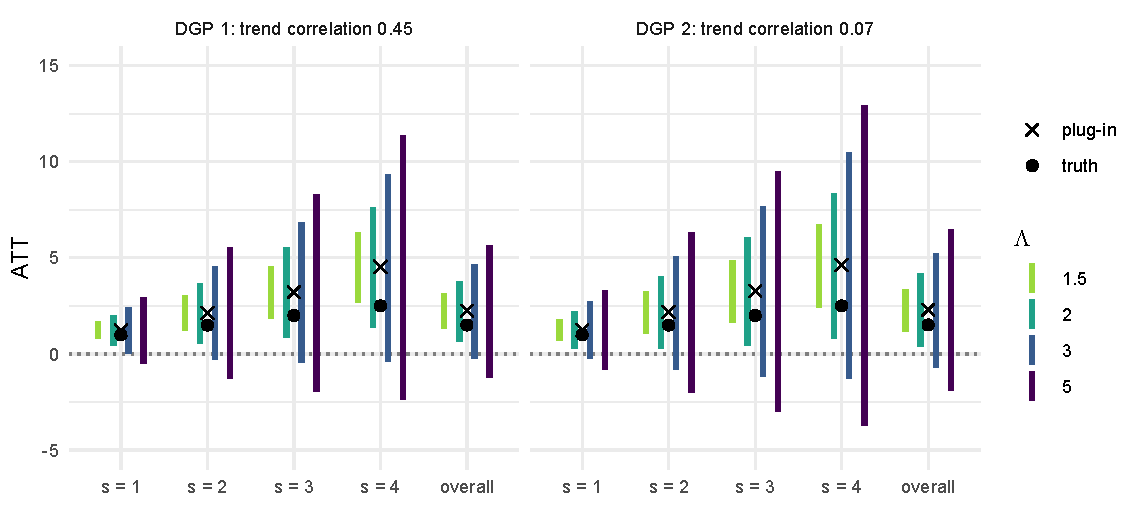
\includegraphics[width=\textwidth]{fig_lambda.pdf}
\caption{Bounds for the four dynamic effects and the overall effect as $\Lambda$
increases, averaged over $150$ replications, for both designs of
Section~\ref{sec:simdesign}. Filled dots mark the true values and crosses the plug-in
estimator, which is the degenerate interval obtained at $\Lambda = 1$ and so is drawn as a
point rather than a bar. The gap between cross and dot is the bias induced by the
violation of parallel trends.}
\label{fig:lambda}
\end{figure}

Figure~\ref{fig:lambda} shows the same information. The plug-in sits above the truth at
every target and increasingly so with duration; the intervals are nested in $\Lambda$ by
construction; and the vertical extent grows with duration at every $\Lambda$, so the
longest-duration effect is hardest to defend even though its point estimate is the
largest. The two panels, drawn on a common scale, differ in the width of the bounds but
not in shape, so the pattern is at least not specific to one of the two designs.

\subsection{Calibration}
\label{sec:simcal}

In DGP~1, over $60$ replications, $\widehat\Lambda_{\mathrm{pre}}(0.95)$ of
\eqref{eq:lampre} has mean $1.379$ and standard deviation $0.088$, and
$\widehat\Lambda_{\Delta,\mathrm{pre}}(0.95)$ of \eqref{eq:lamDpre} has mean
$1.248$ and standard deviation $0.088$. In DGP~2, over $40$ replications, the
corresponding figures are $1.320$ ($0.095$) and $1.294$ ($0.081$). All four are estimated
stably; at $T = 4$ the coherence quantity draws on three cohort-period pairs.

The comparison with Table~\ref{tab:cover} is instructive and not entirely comfortable.
Coverage requires $\Lambda \approx 2$ in both designs, while the pre-adoption departure
visible in the data is $1.38$ and $1.32$ respectively, so the implied multiple is
$M \approx 1.45$ and $1.52$: post-adoption selection must be allowed to be about half
again as strong as the selection observable before adoption. Reporting at $M = 1$ would
have undercovered at the longer durations in both cases. This illustrates the
extrapolation that Section~\ref{sec:testable} flags as an assumption rather than a
deduction. That the two designs agree closely on $M$ is consistent with the risk-set
argument of Section~\ref{sec:testable}, since in both the coefficient on the latent
declines across cohorts, but two designs sharing that feature cannot establish how general
the shortfall is. It does argue for reporting a grid in $M$ rather than a single
calibrated value.

\subsection{Coherence and the correlation of untreated trends}
\label{sec:simcoh}

Section~\ref{sec:range} motivated the coherence constraints by observing that, without
them, a unit's departure may reverse between adjacent periods, so that the worst case
extracts something like $\sum_k |\Delta Y_{ik}|$ where a coherent mechanism would yield
only $|\sum_k \Delta Y_{ik}|$. That reasoning predicts the gain should depend on how
correlated untreated trends are across periods: when they share a driver the two
quantities are close and coherence buys little. The two designs of
Section~\ref{sec:simdesign} were built to test exactly this: they are matched on selection
strength and differ only in the mean pairwise correlation of untreated trends, $0.45$
against $0.07$.

\begin{table}[ht]
\centering
\begin{tabular}{lrrcrrr}
\toprule
& \multicolumn{2}{c}{width reduction (\%)} & & \multicolumn{3}{c}{excludes zero (fraction)}\\
\cmidrule(lr){2-3}\cmidrule(lr){5-7}
& $\Lambda_\Delta = 1.25$ & $\Lambda_\Delta = 1$ & &
  $\Lambda_\Delta = \Lambda^2$ & $\Lambda_\Delta = 1.25$ & $\Lambda_\Delta = 1$\\
\midrule
\multicolumn{7}{@{}l}{\emph{DGP 1: mean pairwise trend correlation $0.45$}}\\
$s = 1$   & 0.0  & 0.1  & & 0.64 & 0.64 & 0.64\\
$s = 2$   & 10.7 & 12.5 & & 0.00 & 0.32 & 0.36\\
$s = 3$   & 14.8 & 17.4 & & 0.00 & 0.72 & 0.88\\
$s = 4$   & 16.6 & 19.9 & & 0.08 & 0.96 & 1.00\\
overall   & 14.5 & 17.1 & & 0.00 & 0.92 & 1.00\\
\midrule
\multicolumn{7}{@{}l}{\emph{DGP 2: mean pairwise trend correlation $0.07$}}\\
$s = 1$   & 0.0  & 0.1  & & 0.00 & 0.00 & 0.00\\
$s = 2$   & 18.5 & 21.4 & & 0.00 & 0.05 & 0.15\\
$s = 3$   & 26.0 & 30.7 & & 0.00 & 0.50 & 0.85\\
$s = 4$   & 29.4 & 35.2 & & 0.00 & 0.90 & 1.00\\
overall   & 26.0 & 30.7 & & 0.00 & 0.80 & 0.90\\
\bottomrule
\end{tabular}
\caption{Effect of the coherence constraints \eqref{eq:coherence} at $\Lambda = 3$,
relative to the uncoupled specification $\Lambda_\Delta = \Lambda^2$. $25$ replications
for DGP~1, $20$ for DGP~2, slack $c_n = 2$.}
\label{tab:coh}
\end{table}

\begin{figure}[ht]
\centering
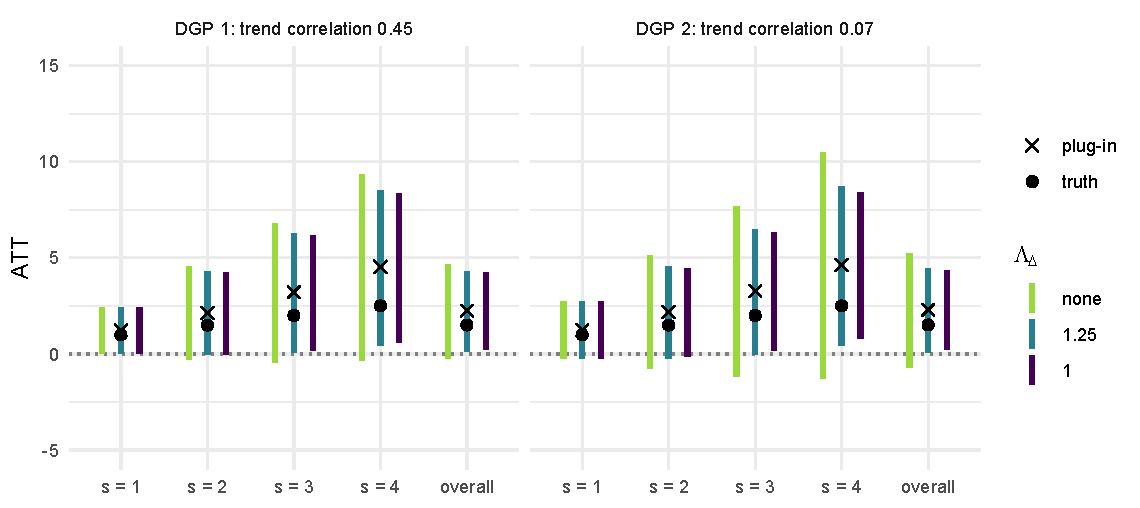
\includegraphics[width=\textwidth]{fig_coherence.pdf}
\caption{Bounds at $\Lambda = 3$ under three values of the coherence parameter, averaged
over replications; ``none'' is the neutral value $\Lambda_\Delta = \Lambda^{2}$. The
vertical scale and markers are as in Figure~\ref{fig:lambda}: filled dots the true
values, crosses the plug-in. The
plug-in does not depend on $\Lambda_\Delta$, since at $\Lambda = 1$ every deviation ratio
equals one and \eqref{eq:coherence} is slack. Coherence bites harder in the right-hand
panel, where untreated trends are nearly independent across periods.}
\label{fig:coh}
\end{figure}

Table~\ref{tab:coh} and Figure~\ref{fig:coh} report both designs at $\Lambda = 3$, the
smallest grid value at which the uncoupled bounds for the overall effect and for
$s \ge 2$ exclude zero in at most $8\%$ of replications. Within each design the
pattern is as Remark~\ref{rmk:couple} anticipates: duration $s = 1$ is untouched, there
being a single borrowing period and nothing to cohere, and the reduction grows with
duration thereafter.

Across designs the results are in the predicted direction. At $\Lambda_\Delta = 1$ the
width reduction at $s = 4$ is $19.9\%$ under correlated trends and $35.2\%$ under weakly
correlated ones; for the overall effect, $17.1\%$ against $30.7\%$. This is consistent
with the value of the coherence assumption depending on a feature of the data that can be
inspected before the assumption is imposed, which is a reason to report the trend
correlation alongside the bounds, though two designs differing in one feature cannot rule
out other explanations. The exclude-zero fractions
are less informative for the cross-design comparison, since DGP~2 starts from bounds about
a fifth wider; within each design they rise steeply with $\Lambda_\Delta$, from essentially
zero to $0.9$ or more at $s = 4$ and for the overall effect.

Two cautions. Coherence recovers power but not precision: under $\Lambda_\Delta = 1$,
which forces a single unit-level departure common to every period, the mean $s = 4$ width
in DGP~2 is still $7.6$, three times the true effect. And coverage remained at $1.00$
throughout, in both designs and at every $\Lambda_\Delta$, including where coherence was
imposed on a design whose departures are not coherent. We had expected a false coherence assumption to cost
coverage; at $\Lambda = 3$ the box appears wide enough to absorb it. The risk should not
be dismissed on this evidence, since a design with $\Lambda$ near the coverage boundary is
where it would show, and we have not examined one.

Finally, $\widehat\Lambda_{\Delta,\mathrm{pre}}$ barely distinguished the two designs,
taking the value $1.29$ (s.d.\ $0.08$) in DGP~2 against $1.25$ (s.d.\ $0.09$) in DGP~1,
despite the very different coherence of the underlying mechanisms. Two effects appear to
offset: departures in DGP~2 vary more across periods, but each is diluted by the averaging
in the assignment rule. The diagnostic is thus weaker than its definition \eqref{eq:lamDpre}
might suggest.

\section{Discussion}
\label{sec:disc}

The method bounds the dynamic and overall effects by letting the odds of adopting at $g$
rather than remaining untreated depend on the untreated trend, and optimising each
estimand over every such mechanism consistent with the observed data. Because both
estimands are affine in those odds, the bounds solve linear programs; they are sharp at
the population level for a rich enough balance class, and valid outer bounds otherwise.

\subsection{Choosing the parameters}
\label{sec:choosing}

Table~\ref{tab:params} collects the quantities an analyst must set. The first three cost
credibility, in the sense that a reader may reasonably dispute them; $\eta$ belongs with
them because \eqref{eq:latentpos} is an untestable overlap condition. The remainder impose
no population restriction, though they carry finite-sample consequences---instability,
lost feasibility, and different reported widths---so $\mathcal{H}$ in particular should be
pre-specified.

\begin{table}[ht]
\centering
\small
\begin{tabular}{@{}l p{3.9cm} p{2.4cm} p{5.1cm}@{}}
\toprule
& Restricts & Range (neutral value) & How to choose \\
\midrule
\multicolumn{4}{@{}l}{\emph{Sensitivity parameters: require justification}}\\[3pt]
$\Lambda$ &
the factor by which the untreated trend may move adoption odds away from what covariates
alone predict &
$\ge 1$ \newline ($\Lambda = 1$ is parallel trends) &
report a grid and the breakdown point $\Lambda^{*}$; anchor with
$\widehat\Lambda_{\mathrm{pre}}$ and show $M = \Lambda/\widehat\Lambda_{\mathrm{pre}}$
over roughly $[1,2]$ \\[12pt]
$\Lambda_\Delta$ &
how fast that departure may change between adjacent borrowing periods &
$[1, \Lambda^{2}]$ \newline ($\Lambda^{2}$ is no restriction) &
always report $\Lambda^{2}$; for tighter values use $\widehat\Lambda_{\Delta,\mathrm{pre}}$,
and label any conclusion that depends on them \\
\midrule
\multicolumn{4}{@{}l}{\emph{Alternative to $\Lambda$ when no model is fitted}}\\[3pt]
$\eta$ &
latent lower bound on cohort probabilities given covariates \emph{and} the period-$k$
untreated trend, per \eqref{eq:latentpos} &
$(0, 1/(T{+}1))$ &
no data-based rule is available, since observed cohort shares do not inform latent
conditional overlap; the smallest plausible share is a heuristic starting point. Uses no
nuisance model, and approaches the $\Lambda \to \infty$ limit as $\eta \to 0$ \\
\midrule
\multicolumn{4}{@{}l}{\emph{Tuning and modelling choices: no extra population restriction}}\\[3pt]
$\mathcal{H}$ &
nothing---enlarging it tightens the bounds without new assumptions &
finite, with $1 \in \mathcal{H}$ &
pre-specify a nested ladder and report every rung alongside its feasibility count \\[12pt]
$c_n$ &
slack in the moment constraints, in standard errors per moment, per \eqref{eq:slack} &
$\ge 0$, $c_n = o(\sqrt{n})$ \newline ($0$ is exact equality) &
fix at $2$; a tuning constant, not a sensitivity parameter. Larger values widen the bounds
slightly and improve feasibility; the population bounds do not depend on it. Avoid $0$,
which makes the truth infeasible and can lose coverage at the boundary $\Lambda$ \\[12pt]
$q$ &
trimming level of the calibration quantities &
$(0,1)$ &
$0.95$, checking $0.90$ and $0.99$; affects the reported scale, not the bounds \\
\bottomrule
\end{tabular}
\caption{Quantities the analyst specifies, and how to set them.}
\label{tab:params}
\end{table}

Two points deserve emphasis. First, $\Lambda$ should be reported on a grid led by the
breakdown point $\Lambda^{*}$; the simulation cautions against mechanical calibration,
since in both designs $\widehat\Lambda_{\mathrm{pre}} \approx 1.35$ while coverage
required $\Lambda \approx 2$. Second, the neutral value $\Lambda_\Delta = \Lambda^{2}$
should always appear alongside any tighter choice. Constraint \eqref{eq:coherence} is an
assumption the data cannot check in the periods where it is used, and its effect can be
material: in Section~\ref{sec:sim} it moved the longest-duration and overall bounds from
almost never excluding zero to doing so in most replications, in both designs.

\subsection{What the inference does not yet deliver}

Theorem~\ref{thm:valid} establishes that the bounds are consistent for the identified set,
converging at the rate $(1 \vee c_n)\,n^{-1/2}$ without any uniqueness condition on the dual, and
asymptotically contain the estimand whenever it lies in the interior of that set. That is
not a confidence set. The
Imbens--Manski interval of Section~\ref{sec:practical} supplies one, subject to the
uniformity caveat of \citet{stoye2009more} and pointwise in the target, and
Table~\ref{tab:cover} likewise reports pointwise coverage; a simultaneous band over the
event-study profile requires a multiplicity adjustment we have not developed.
This is the dimension on which \citet{rambachan2023honest} are furthest ahead, offering
procedures with uniform validity over their restriction set.

Two further gaps are asymptotic. Theorem~\ref{thm:valid} requires $\mathcal{H}$ finite
while Theorem~\ref{prop:sharp} requires it to span $L_2(P_X)$, and the sieve rate
$J_n \to \infty$ reconciling them---a growing-dimension convex M-estimation
problem---remains to be worked out. And the calibration quantities \eqref{eq:lampre} and
\eqref{eq:lamDpre} should be root-$n$ estimable and asymptotically normal under standard
conditions on the first-stage fits, but this has not been established, and the maximum
over $(g,k)$ introduces a boundary problem when several pairs are near the maximum.

\subsection{What the restriction does not capture}

The sharpest limitation is that the cross-period restriction is blunt. Much of the power
of \citet{rambachan2023honest} comes from bounding second differences of the violation
path; \eqref{eq:coherence} bounds ratios of adjacent departures instead, and in
Section~\ref{sec:sim} recovers between eleven and thirty-five per cent of width at
durations $s \ge 2$, the larger figure only when untreated trends are close to independent
across periods. Whether a
second-difference analogue can be expressed linearly in $a$---so preserving the linear
program---is the most valuable open question here, because without it the bounds widen
roughly linearly in the duration (Proposition~\ref{prop:closed}) and long-horizon
event-study estimates are likely to remain uninformative at credible values of $\Lambda$,
as they were in our designs.

The calibration of $\Lambda_\Delta$ is correspondingly thin. The pre-adoption coherence
\eqref{eq:lamDpre} draws on only $(T{-}1)(T{-}2)/2$ cohort-period pairs, and
Section~\ref{sec:simcoh} found it barely able to distinguish two designs whose departures
differ sharply in coherence; the correlation of untreated trends, which tracked the gain in
those designs, appears to be the more informative diagnostic. More fundamentally, the gap
between the calibrated $M = 1$ and the $M \approx 1.5$ needed for coverage in both designs
illustrates that the extrapolation from pre- to post-adoption selection need not be
innocuous. Part of it is mechanical, for the risk-set reason
of Section~\ref{sec:testable}; how much is mechanical and how much reflects genuine
differences between pre- and post-adoption selection has not been separated. Until it is,
pre-period calibration should inform the grid rather than replace it.

Two structural restrictions are worth restating. Sharpness holds for a model posited
period by period; bounding the mechanism conditional on the whole trend path would be
sharp for a path-level restriction, but that path is censored at adoption, so only
never-treated units contribute complete paths, apparently forcing a trade-off between
sharpness under that model and the pooling of not-yet-treated cohorts. And no anticipation
is maintained throughout: it contaminates the base period $Y_{g-1}$ rather than the
borrowed trends, and the present analysis says nothing about it.

\subsection{Extensions}

The restriction to baseline covariates is inessential: carrying a period index through the
propensity score, so that $a_{g,k}$ becomes a function of $X_k$, delivers the same
construction under an exogeneity condition on the covariate path. A precise comparison
with \citet{rambachan2023honest} on common data would be more valuable still, since the
two approaches restrict different objects and draw on different information, and which is
more informative in practice is an empirical question we have not settled.

\appendix
\section{Proofs and auxiliary results}
\label{app:proofs}

\setcounter{lemma}{0}
\renewcommand{\thelemma}{A\arabic{lemma}}
\setcounter{proposition}{0}
\renewcommand{\theproposition}{A\arabic{proposition}}
\setcounter{corollary}{0}
\renewcommand{\thecorollary}{A\arabic{corollary}}
\setcounter{remark}{0}
\renewcommand{\theremark}{A\arabic{remark}}
% hyperref anchors must be renamed too, or appendix results collide with main-text ones
\renewcommand{\theHlemma}{A\arabic{lemma}}
\renewcommand{\theHproposition}{A\arabic{proposition}}
\renewcommand{\theHcorollary}{A\arabic{corollary}}
\renewcommand{\theHremark}{A\arabic{remark}}

\subsection{Aggregation and the odds representation}

\begin{lemma}[Aggregation]
\label{lem:agg}
Identity \eqref{eq:agg} holds.
\end{lemma}

\begin{proof}
The cell $(g,t)$ lies on the diagonal $s = t-g+1$, and diagonal $s$ consists of the cells
$(g, g+s-1)$ with $g \le T-s+1$, so the triangle partitions into its diagonals.
Substituting \eqref{eq:dyn} into the numerator of \eqref{eq:overall} gives the first
claim. For the second,
$\sum_{s=1}^{T} P(G \le T{-}s{+}1) = \sum_{g=1}^{T} P(G{=}g)\,\#\{s : s \le T{-}g{+}1\}$.
\end{proof}

\begin{lemma}[Reweighting identity]
\label{lem:reweight}
Under Assumption~\ref{ass:pos}, identity \eqref{eq:reweight} holds for any integrable
$\psi$ and any $g \le k$.
\end{lemma}

\begin{proof}
Conditioning on $X$ inside the right-hand side,
\[
E\{I(G>k) a_{g,k}(X)\psi(X)\} = E\{P(G>k \mid X)\, a_{g,k}(X)\,\psi(X)\}
 = E\{P(G{=}g \mid X)\psi(X)\},
\]
which equals $E\{I(G{=}g)\psi(X)\}$, that is,
$P(G{=}g)E\{\psi(X) \mid G{=}g\}$. Positivity makes the denominator of
\eqref{eq:odds} nonzero.
\end{proof}

\begin{proof}[Proof of Proposition~\ref{prop:oddsrep}]
Apply \eqref{eq:reweight} with $\psi = \delta_k$ to the outer average in
\eqref{eq:identreg}. Since $\delta_k(X) = E\{\Delta Y_k \mid X, G > k\}$, the tower
property gives
\[
E\{I(G{>}k)\,a_{g,k}(X)\,\delta_k(X)\} = E\{I(G{>}k)\,a_{g,k}(X)\,\Delta Y_k\},
\]
and substituting into \eqref{eq:identreg} yields \eqref{eq:oddsrep}.
\end{proof}

\subsection{Identification without parallel trends}

\begin{proof}[Proof of Lemma~\ref{lem:restore}]
Write $Z = (X, \Delta Y_k(\infty))$. Both sides are finite: the right by hypothesis, and
the left because, by the computation below applied to $|\psi|$, it equals the right with
$|\psi|$ in place of $\psi$. Conditioning on $Z$ and using that $\alpha_{g,k}(Z)\psi(Z)$
is $Z$-measurable,
\begin{align*}
E\{I(G{>}k)\,\alpha_{g,k}(Z)\,\psi(Z)\}
&= E\big[ P(G{>}k \mid Z)\,\alpha_{g,k}(Z)\,\psi(Z) \big]\\
&= E\big[ P(G{=}g \mid Z)\,\psi(Z) \big]
= E\{I(G{=}g)\,\psi(Z)\},
\end{align*}
the second equality because $P(G{>}k \mid Z) > 0$ on the support of $Z$ given $G = g$ by
the finiteness condition of Section~\ref{sec:model}, so that
$P(G{>}k \mid Z)\,\alpha_{g,k}(Z) = P(G{=}g \mid Z)$ there, while off that support
$P(G{=}g \mid Z) = 0$ and the right-hand integrand vanishes.
\end{proof}

\begin{proof}[Proof of Proposition~\ref{prop:ident}]
By Assumption~\ref{ass:na}, $Y_{g-1}(g) = Y_{g-1}(\infty)$, and by
Assumption~\ref{ass:cons}, $Y_r = Y_r(g)$ and $Y_{g-1} = Y_{g-1}(\infty)$ on $\{G = g\}$.
Hence
\[
E(Y_r - Y_{g-1} \mid G{=}g) - \tau_{g,r}
= E\{Y_r(\infty) - Y_{g-1}(\infty) \mid G{=}g\}
= \sum_{k=g}^{r} E\{\Delta Y_k(\infty) \mid G{=}g\}.
\]
For a unit with $G > k$, Assumptions~\ref{ass:cons} and~\ref{ass:na} give
$\Delta Y_k = \Delta Y_k(\infty)$, so
\[
I(G{>}k)\,\alpha_{g,k}(X, \Delta Y_k(\infty))\,\Delta Y_k
 = I(G{>}k)\,\alpha_{g,k}(X, \Delta Y_k(\infty))\,\Delta Y_k(\infty),
\]
and Lemma~\ref{lem:restore} with $\psi(X,\delta) = \delta$, which is applicable because
$E\{I(G{=}g)|\Delta Y_k(\infty)|\} < \infty$ whenever $\tau_{g,r}$ is defined, gives
$E\{I(G{>}k)\,\alpha_{g,k}\,\Delta Y_k\} = P(G{=}g)\,E\{\Delta Y_k(\infty) \mid G{=}g\}$.
Substituting into the display yields \eqref{eq:identsens}.
\end{proof}

\subsection{Dual representation and proof of Theorem~\ref{thm:valid}}

\begin{lemma}[Dual representation]
\label{lem:dual}
In the notation of Section~\ref{sec:valid}, write \eqref{eq:lp} as
$\max_a \sum_\iota c_\iota a_\iota$ subject to $\sum_\iota M_{j\iota} a_\iota = m_j$,
$j = 1, \ldots, J'$, and $a_i \in \mathcal{B}_i$ for every $i$, where
$M_{j\iota} = h(X_i)I(G_i > k)$ when the cohort-period labels of $j = (h,g,k)$ and
$\iota = (i,g,k)$ agree and zero otherwise, and $m_j = \sum_i I(G_i{=}g)h(X_i)$. If the
program is feasible, its optimal value equals
$n \min_{\lambda \in \mathbb{R}^{J'}} \mathbb{P}_n \phi(\cdot\,;\lambda)$ with $\phi$ as
in \eqref{eq:dualphi}. For the slackened program \eqref{eq:slack} the
representation holds with $\phi(O_i;\lambda)$ replaced by
$\phi(O_i;\lambda) + (c_n/\sqrt{n})\,\|\lambda\|_{1,\widehat s}$. When $\Lambda_\Delta = \Lambda^2$,
$\sigma_i(v) = \sum_{g \le k} \{ (v_{g,k})_+\, u_{i,g,k} + (v_{g,k})_-\, \ell_{i,g,k} \}$
with $z_+ = \max(z,0)$ and $z_- = \min(z,0)$.
\end{lemma}

\begin{proof}
Each $\mathcal{B}_i$ is a polytope, so the primal is a finite linear program; its feasible
set is compact, so the optimal value is finite when it is nonempty. For fixed $\lambda$ the
partial Lagrangian, dualising only the moment equations, is
\[
\sum_\iota c_\iota a_\iota - \sum_j \lambda_j\Big(\sum_\iota M_{j\iota}a_\iota - m_j\Big)
= \sum_j \lambda_j m_j + \sum_i \sum_{g \le k}\big(c_{i,g,k} - \xi_{i,g,k}(\lambda)\big)\,a_{i,g,k},
\]
since $\sum_j \lambda_j M_{j\iota} = I(G_i{>}k)\sum_h \lambda_{h,g,k}h(X_i) = \xi_{i,g,k}(\lambda)$
for $\iota = (i,g,k)$. Maximising over $a \in \prod_i \mathcal{B}_i$ separates across
units and gives $\sum_j \lambda_j m_j + \sum_i \sigma_i(c_i - \xi_i(\lambda))$, which is
$\sum_i \phi(O_i;\lambda) = n\,\mathbb{P}_n\phi(\cdot;\lambda)$ because
$\sum_j \lambda_j m_j = \sum_i \sum_{(h,g,k)} \lambda_{h,g,k} I(G_i{=}g)h(X_i)$. Weak
duality, primal value $\le \min_\lambda n\mathbb{P}_n\phi(\cdot;\lambda)$, is immediate.
For equality, write the polytope constraints $a_i \in \mathcal{B}_i$ as finitely many
linear inequalities $R a \le r$; by linear programming duality (feasible and bounded primal)
the full dual $\min\{\lambda' m + \nu' r : \nu \ge 0,\ M'\lambda + R'\nu = c\}$ has the
same value, and minimising over $\nu$ at fixed $\lambda$ recovers
$\max_{a \in \prod \mathcal{B}_i}\sum_\iota (c - M'\lambda)_\iota a_\iota$ by duality for
the inner bounded linear program, so the partial dual has zero gap. Under \eqref{eq:slack}
each equality becomes two inequalities
$\pm\big(\sum_\iota M_{j\iota}a_\iota - m_j\big) \le c_n\sqrt{n}\,\widehat s_j$ with
multipliers $\lambda_j^{\pm} \ge 0$; writing $\lambda_j = \lambda_j^{+} - \lambda_j^{-}$
the dual objective becomes
$\lambda' m + c_n\sqrt{n}\sum_j \widehat s_j(\lambda_j^{+} + \lambda_j^{-}) + \cdots$,
minimised at $\lambda_j^{+} + \lambda_j^{-} = |\lambda_j|$, which after division by $n$
gives the penalty $(c_n/\sqrt{n})\|\lambda\|_{1,\widehat s}$. The minimisation problems in \eqref{eq:lp}
are covered on replacing $c$ by $-c$. The box case of $\sigma_i$ is immediate, each
coordinate being maximised separately.
\end{proof}

\begin{proof}[Proof of Theorem~\ref{thm:valid}]
We treat the upper bound; the lower bound follows on replacing the objective by its
negative. Write $d = T(T{+}1)/2$ for the number of cohort-period pairs.

\emph{Step 0: reduction and notation.} The objective coefficients in \eqref{eq:objdyn} and
\eqref{eq:objoverall} have the form $c_{i,g,k} = \tilde c_{g,k}(O_i)/N_\bullet$ with
\[
\tilde c_{g,k}(O) = -\,I(G{>}k)\,\Delta Y_k\, r_\bullet(g,k),
\qquad
r_{\mathrm{dyn}_s}(g,k) = I\{g \in \mathcal{W}^{(s)}_k\},\quad
r_{\mathrm{overall}}(g,k) = T-k+1,
\]
and $N_\bullet \in \{N_s, N_D\}$. Then $\widehat\Theta^{+} = C_\bullet/N_\bullet +
(n/N_\bullet)\,\widehat V$, where $\widehat V$ is $n^{-1}$ times the optimal value of the
program with coefficients $\tilde c$, and $\Theta^{+} = \bar C_\bullet/p_\bullet +
V/p_\bullet$, where $\bar C_\bullet$ and $p_\bullet$ are the population limits of
$C_\bullet/n$ and $N_\bullet/n$ and
\begin{multline*}
V = \sup\Big\{ E\Big[\sum_{g \le k} \tilde c_{g,k}(O)\,\alpha_{g,k}\Big] :\
 \alpha \in \mathcal{B} \text{ a.s.},\\
 E\{I(G{>}k)\,\alpha_{g,k}\,h(X)\} = E\{I(G{=}g)h(X)\}
 \text{ for all } (h,g,k) \Big\},
\end{multline*}
with $\alpha_{g,k}$ short for $\alpha_{g,k}(X, \Delta Y_k(\infty))$ and, in the anchored
case, $\mathcal{B}$ centred at $\bar a$. Since $C_\bullet/N_\bullet \to \bar C_\bullet/p_\bullet$
and $N_\bullet/n \to p_\bullet > 0$ in probability, each with $O_p(n^{-1/2})$ error by the
central limit theorem and Assumption~\ref{ass:reg}(iii), it suffices to prove (ii) and (iv)
for $\widehat V$ and $V$. Let $\phi(O;\lambda)$ denote \eqref{eq:dualphi} with $\tilde c$
in place of $c$ and, in the anchored case, with the population polytope
$\bar{\mathcal{B}}(O)$ centred at $\bar a(X)$; let $\widehat\phi(O_i;\lambda)$ denote the
same function with the sample polytope $\mathcal{B}_i$ centred at $\widehat a(X_i)$. By
Lemma~\ref{lem:dual},
\[
\widehat V = \min_{\lambda \in \mathbb{R}^{J'}} \Psi_n(\lambda),
\qquad
\Psi_n(\lambda) = \mathbb{P}_n \widehat\phi(\cdot;\lambda) + \frac{c_n}{\sqrt n}\|\lambda\|_{1,\widehat s} .
\]
Since $\widehat s_{h,g,k}^{\,2} \le \mathbb{P}_n h(X)^2 (\bar c + 1)^2 = O_p(1)$ and
$\widehat s_{h,g,k}$ is bounded below as noted after \eqref{eq:slack},
$\|\lambda\|_{1,\widehat s}$ is equivalent to $\|\lambda\|_1$ up to $O_p(1)$ constants, and
we treat it as such below.

\emph{Step 1: properties of $\phi$.} For fixed $O$, $\lambda \mapsto \phi(O;\lambda)$ is
convex, being a linear function plus the composition of a support function---convex and
positively homogeneous---with an affine map. Since $\mathcal{B}(O) \subset
[\underline c, \bar c]^{d}$, its support function satisfies
$|\sigma(v) - \sigma(v')| \le \bar c\,\|v - v'\|_1$. Hence
\[
|\phi(O;\lambda) - \phi(O;\lambda')| \le L(O)\,\|\lambda - \lambda'\|_\infty,
\qquad
L(O) = (1 + \bar c)\, d \sum_{j=1}^{J} |h_j(X)|,
\]
and $|\phi(O;\lambda)| \le \bar c\,\|\tilde c(O)\|_1 + L(O)\|\lambda\|_\infty$ with
$\|\tilde c(O)\|_1 \le T d \sum_k |\Delta Y_k|$. By Assumption~\ref{ass:reg}(i) and (iii),
$E\{L(O)^2\} < \infty$ and $E\{\|\tilde c(O)\|_1^2\} < \infty$, so on every compact
$K \subset \mathbb{R}^{J'}$ the class $\{\phi(\cdot;\lambda) : \lambda \in K\}$ has a
square-integrable envelope and is Lipschitz in $\lambda$ with square-integrable Lipschitz
constant.

\emph{Step 2: population duality and the dual argmin.} Let $\mathcal{M}$ and $m^0 =
(E\{I(G{=}g)h(X)\})_{(h,g,k)}$ be as in Assumption~\ref{ass:slater}, and for $m \in \mathcal{M}$
let $V(m)$ be the supremum defining $V$ with $m$ in place of $m^0$, so that $V = V(m^0)$.
The set $\mathcal{M}$ is convex and $V$ is finite and concave on it: if $\alpha^1, \alpha^2$
are feasible for $m^1, m^2$ then $t\alpha^1 + (1{-}t)\alpha^2 \in \mathcal{B}$ almost surely
is feasible for $tm^1 + (1{-}t)m^2$, and the objective is linear; finiteness follows from
$|E\sum \tilde c_{g,k}\alpha_{g,k}| \le \bar c\,E\|\tilde c\|_1 < \infty$. For any $\lambda$
and any $\alpha$ feasible for $m^0$,
\[
E\Big[\sum_{g \le k}\tilde c_{g,k}\alpha_{g,k}\Big]
= \lambda' m^0 + E\Big[\sum_{g \le k}\big(\tilde c_{g,k} - \xi_{g,k}(\lambda)\big)\alpha_{g,k}\Big]
\le \lambda' m^0 + E\,\sigma\big(\tilde c - \xi(\lambda)\big) = P\phi(\cdot;\lambda),
\]
where $\xi_{g,k}(\lambda) = I(G{>}k)\sum_h \lambda_{h,g,k}h(X)$, so
$V \le \inf_\lambda P\phi(\cdot;\lambda)$. Conversely, because $m^0$ is an interior point
of $\mathcal{M}$, the concave function $V$ has a nonempty compact set $\mathcal{L}^*$ of
supergradients at $m^0$ \citep[Theorem~23.4]{rockafellar1970convex}. For $\lambda^* \in
\mathcal{L}^*$ and any $\alpha \in \mathcal{B}$ almost surely, with moment vector
$m = E\{I(G{>}k)\alpha_{g,k}h(X)\} \in \mathcal{M}$,
\[
E\Big[\sum_{g \le k}\tilde c_{g,k}\alpha_{g,k}\Big] \le V(m) \le V(m^0) + \lambda^{*\prime}(m - m^0),
\]
that is,
\[
E\Big[\sum_{g \le k}\big(\tilde c_{g,k} - \xi_{g,k}(\lambda^*)\big)\alpha_{g,k}\Big] \le V - \lambda^{*\prime}m^0 .
\]
Taking the supremum over such $\alpha$---the pointwise maximiser of a linear functional
over $\mathcal{B}(O)$ can be chosen as a vertex in a fixed enumeration, hence
measurably---gives $E\sigma(\tilde c - \xi(\lambda^*)) \le V - \lambda^{*\prime}m^0$, that
is $P\phi(\cdot;\lambda^*) \le V$. Hence $V = \min_\lambda P\phi(\cdot;\lambda)$, the
minimum is attained exactly on $\mathcal{L}^*$, and since $\lambda \mapsto P\phi(\cdot;\lambda)$
is a finite convex function with nonempty bounded argmin, all of its level sets are bounded
\citep[Corollary~8.7.1]{rockafellar1970convex}.

\emph{Step 3: proof of (i).} At $\alpha^0$ the left side of \eqref{eq:slack} is
$\mathbb{P}_n\{h(X)(I(G{>}k)\alpha^0_{g,k} - I(G{=}g))\}$, an average of independent terms
with mean zero by Lemma~\ref{lem:restore} and variance at most $(\bar c + 1)^2 E\{h(X)^2\}
< \infty$; hence it is $O_p(n^{-1/2})$. The right side is $c_n\widehat s_{h,g,k}/\sqrt n$
with $\widehat s_{h,g,k}$ bounded below in probability by a positive constant, so a union
bound over the $J'$ constraints together with $c_n \to \infty$ shows that the moment part
of $\widehat{\mathcal{A}}_n$ holds at $\alpha^0$ with probability tending to one. In the absolute case $\alpha^0 \in \mathcal{B}_i$
by hypothesis. In the anchored case let $\epsilon_n = \max_{i,g,k}|\widehat a_{g,k}(X_i)/
\bar a_{g,k}(X_i) - 1| \to 0$ in probability by Assumption~\ref{ass:reg}(iv), and let $D_i$
be the diagonal matrix with entries $\widehat a_{g,k}(X_i)/\bar a_{g,k}(X_i)$. Every
inequality in \eqref{eq:lambdabox} and \eqref{eq:coherence} is homogeneous of degree one in
the centres, so $\mathcal{B}_i = D_i\bar{\mathcal{B}}_i$, and $\alpha^0_i \in \mathcal{B}_i$
if and only if $D_i^{-1}\alpha^0_i \in \bar{\mathcal{B}}_i$. Rescaling coordinates by
factors in $[(1{+}\epsilon_n)^{-1}, (1{-}\epsilon_n)^{-1}]$ changes each box ratio
$\alpha_{g,k}/\bar a_{g,k}$ by a factor in that interval and each coherence ratio by a
factor in $[(1{-}\epsilon_n)/(1{+}\epsilon_n), (1{+}\epsilon_n)/(1{-}\epsilon_n)]$. By the
margin hypothesis the ratios at $\alpha^0$ lie within $(1{-}\epsilon)\Lambda$ and
$(1{-}\epsilon)\Lambda_\Delta$ of their centres, so $D_i^{-1}\alpha^0_i \in \bar{\mathcal{B}}_i$
for every $i$ as soon as $(1{-}\epsilon)(1{+}\epsilon_n)/(1{-}\epsilon_n) \le 1$, an event
whose probability tends to one.

\emph{Step 4: proof of (ii).} Fix a compact $K \subset \mathbb{R}^{J'}$. By Step~1 and the
strong law, $\mathbb{P}_n\phi(\cdot;\lambda) \to P\phi(\cdot;\lambda)$ almost surely for
each $\lambda$; since these are finite convex functions of $\lambda$, pointwise convergence
on a countable dense set implies uniform convergence on $K$
\citep[Theorem~10.8]{rockafellar1970convex}. In the anchored case, $\mathcal{B}_i = D_i
\bar{\mathcal{B}}_i$ gives $\widehat\sigma_i(v) = \bar\sigma_i(D_i v)$ for the two support
functions, so $|\widehat\phi(O_i;\lambda) - \phi(O_i;\lambda)| \le \bar c\,\|(D_i - I)
(\tilde c_i - \xi_i(\lambda))\|_1 \le \bar c\,\epsilon_n\,\|\tilde c_i - \xi_i(\lambda)\|_1$,
and averaging, $\sup_{\lambda \in K}|\mathbb{P}_n\widehat\phi - \mathbb{P}_n\phi| \le
\bar c\,\epsilon_n\,\mathbb{P}_n\{\|\tilde c\|_1 + L\sup_K\|\lambda\|_\infty\} = o_p(1)$.
The penalty satisfies $\sup_{K}(c_n/\sqrt n)\|\lambda\|_{1,\widehat s} \to 0$ in
probability. Hence
$\sup_{\lambda \in K}|\Psi_n(\lambda) - P\phi(\cdot;\lambda)| \to 0$ in probability, and
$\Psi_n$ is convex.

Now take $K$ to be the closed unit neighbourhood of $\mathcal{L}^*$ and let $\zeta =
\min_{\lambda \in \partial K} P\phi(\cdot;\lambda) - V$, which is positive because $\partial K$
is compact, disjoint from the argmin set $\mathcal{L}^*$, and $P\phi$ is continuous. On the
event $\sup_K|\Psi_n - P\phi| < \zeta/2$, take any $\lambda \notin K$ and $\lambda^* \in
\mathcal{L}^*$; the segment from $\lambda^*$ to $\lambda$ meets $\partial K$ at some
$\lambda_b = t\lambda^* + (1{-}t)\lambda$ with $t \in (0,1)$, and convexity of $\Psi_n$
gives $\Psi_n(\lambda_b) \le t\Psi_n(\lambda^*) + (1{-}t)\Psi_n(\lambda)$, whence
\[
\Psi_n(\lambda) \ \ge\ \Psi_n(\lambda^*) + \frac{\Psi_n(\lambda_b) - \Psi_n(\lambda^*)}{1-t}
\ \ge\ \Psi_n(\lambda^*) + \big(P\phi(\cdot;\lambda_b) - \zeta/2\big) - \big(V + \zeta/2\big)
\ \ge\ \Psi_n(\lambda^*).
\]
So on that event $\inf_{\mathbb{R}^{J'}}\Psi_n = \min_K \Psi_n$, and therefore
$|\widehat V - V| = |\min_K\Psi_n - \min_K P\phi| \le \sup_K|\Psi_n - P\phi| < \zeta/2$.
Since the event has probability tending to one and $\zeta$ may be replaced by any smaller
positive number, $\widehat V \to V$ in probability.

\emph{Step 5: proof of (iii).} The trend-dependent odds $\alpha$ satisfy the population
moment equations by Lemma~\ref{lem:restore} with $\psi = h$, which is applicable because
$E\{I(G{=}g)|h(X)|\} \le E\{h(X)^2\}^{1/2} < \infty$, and lie in $\mathcal{B}$ almost
surely by hypothesis; so $\alpha$ is feasible for the population program, and by
Proposition~\ref{prop:ident} the population objective at $\alpha$ equals $\tau^\bullet$.
Hence $\Theta^- \le \tau^\bullet \le \Theta^+$. If the inequalities are strict, (ii) gives
$P(\widehat\Theta^- < \tau^\bullet < \widehat\Theta^+) \to 1$.

\emph{Step 6: proof of (iv).} Suppose $\epsilon_n = O_p(n^{-1/2})$ in the anchored case
and $\epsilon_n = 0$ in the absolute case. For the upper bound fix $\lambda^* \in \mathcal{L}^*$:
\begin{align*}
\widehat V \le \Psi_n(\lambda^*)
&\le \mathbb{P}_n\phi(\cdot;\lambda^*) + \bar c\,\epsilon_n\,\mathbb{P}_n\|\tilde c - \xi(\lambda^*)\|_1
 + \frac{c_n}{\sqrt n}\|\lambda^*\|_{1,\widehat s}\\
&= V + O_p(n^{-1/2}) + O_p(\epsilon_n) + O_p(c_n n^{-1/2}),
\end{align*}
by the central limit theorem for the fixed square-integrable function $\phi(\cdot;\lambda^*)$.
For the lower bound let $\widehat\lambda_n \in \arg\min\Psi_n$, which lies in $K$ with
probability tending to one by Step~4. Then
\begin{align*}
\widehat V = \Psi_n(\widehat\lambda_n)
&\ge \mathbb{P}_n\widehat\phi(\cdot;\widehat\lambda_n)
\ge \mathbb{P}_n\phi(\cdot;\widehat\lambda_n) - O_p(\epsilon_n)\\
&\ge P\phi(\cdot;\widehat\lambda_n) - \sup_{\lambda \in K}|(\mathbb{P}_n - P)\phi(\cdot;\lambda)| - O_p(\epsilon_n)\\
&\ge V - \sup_{\lambda \in K}|(\mathbb{P}_n - P)\phi(\cdot;\lambda)| - O_p(\epsilon_n).
\end{align*}
By Step~1 the class $\{\phi(\cdot;\lambda) : \lambda \in K\}$ is Lipschitz in the
finite-dimensional parameter $\lambda$ with a square-integrable Lipschitz constant, hence
Donsker \citep[Example~19.7]{vandervaart1998asymptotic}, so the supremum is
$O_p(n^{-1/2})$. Combining, $\widehat V = V + O_p\{(1 \vee c_n) n^{-1/2}\}$, and Step~0
transfers the rate to $\widehat\Theta^{+}$. Uniqueness of the dual solution is not
required. Nothing in Steps~4 and~6 uses $c_n > 0$: they need only Lemma~\ref{lem:dual},
which requires the sample program to be feasible, so at $c_n = 0$ they go through under
the stated feasibility hypothesis with the penalty term absent.
\end{proof}

\subsection{Remarks}
\label{app:remarks}

\begin{remark}[Mean versus full independence]
\label{rmk:meanind}
Assumption~\ref{ass:pt} is a mean-independence condition, whereas constancy of
\eqref{eq:tdodds} in $\delta$ for every $g \le k$ is full conditional independence of
$I(G{=}g)$, and hence of $I(G{>}k)$, from $\Delta Y_k(\infty)$ given $X$, which is
stronger than the corresponding mean condition. Letting $\alpha$ vary therefore explores
mean and non-mean departures alike; the bounds are valid for the estimands, though a box
around a fixed $\alpha$ does not correspond exactly to a set of mean violations.
\end{remark}

\begin{remark}[Feasibility at $\Lambda = 1$]
\label{rmk:lambda1}
At $\Lambda = 1$ the box pins $a_{i,g,k} = \widehat a_{g,k}(X_i)$, and the program is
feasible only if the fitted odds satisfy \eqref{eq:moment} in sample. Maximum likelihood
does not deliver this: the logistic score equations are
$\sum_i h(X_i)\{\widehat\pi_g(X_i) - I(G_i{=}g)\} = 0$, which agree with \eqref{eq:moment}
only in the limit under correct specification. Either fit $\widehat a$ by solving
\eqref{eq:moment} directly, in the manner of covariate balancing propensity scores, or use
the slackened program \eqref{eq:slack}, under which the fitted odds clears the constraints
with probability tending to one.
\end{remark}

\begin{remark}[Feasibility monitoring is a constraint qualification check]
\label{rmk:feas}
Assumption~\ref{ass:slater} is what makes the optimal value Lipschitz in the data. When it
nearly fails the dual optimum diverges, the bounds cease to be stable, and bootstrap
replicates begin to be infeasible. The feasibility count recommended in
Section~\ref{sec:practical} is therefore an empirical check on
Assumption~\ref{ass:slater}, not merely a computational diagnostic.
\end{remark}

\begin{remark}[A tension between sharpness and estimability]
\label{rmk:tension}
Theorem~\ref{thm:valid} wants $\mathcal{H}$ finite; Theorem~\ref{prop:sharp} wants it to
span $L_2(P_X)$. The natural resolution is a sieve, $J = J_n \to \infty$ slowly, so the
bounds approach the sharp set while the dual dimension grows slowly enough to preserve
consistency. This also explains the observation of \citet{tang2025simple} that richer
constraint classes give narrower but less stable bounds. The permissible rate is left
open.
\end{remark}

\begin{remark}[Scope of sharpness]
\label{rmk:sharpscope}
Sharpness is relative to a model posited period by period. Bounding instead the path-level
mechanism $P\{G{=}g \mid X, \Delta Y_1(\infty), \ldots, \Delta Y_T(\infty)\}$ would leave
the present program an outer set, since odds do not marginalise linearly. Coherence is
included in the model relative to which sharpness holds only because, as
Section~\ref{sec:range} stresses, it is a restriction on the marginal odds themselves; a
coherence restriction stated at the path level would again leave the program an outer
set. With $\mathcal{H}$ finite the program is likewise an outer set, converging as
$\mathcal{H}$ grows.
\end{remark}

\subsection{Structural properties}
\label{app:struct}

\begin{proposition}[Augmentation is absorbed]
\label{prop:aug}
Let $\widehat\delta_k(X)$ be any estimate of $E\{\Delta Y_k(\infty) \mid X\}$ and replace
$\Delta Y_{ik}$ in \eqref{eq:objdyn} by $\Delta Y_{ik} - \widehat\delta_k(X_i)$, adjusting
the treated-side term correspondingly. If $\widehat\delta_k \in \mathrm{span}(\mathcal{H})$
for every $k$, the optimal value is unchanged; under the slackened program
\eqref{eq:slack} it is unchanged up to $O_p\{(1 \vee c_n) n^{-1/2}\}$.
\end{proposition}

\begin{proof}
The objectives differ by
$N_s^{-1}\sum_k \sum_{g \in \mathcal{W}^{(s)}_k}\sum_{i:G_i>k} a_{i,g,k}\widehat\delta_k(X_i)$
minus the treated-side adjustment. Applying \eqref{eq:moment} with $h = \widehat\delta_k$
turns the first into $\sum_k \sum_{g \in \mathcal{W}^{(s)}_k}\sum_i I(G_i{=}g)\widehat\delta_k(X_i)$,
a constant. For a unit with $G_i = g \le T-s+1$ the periods $k$ with
$g \in \mathcal{W}^{(s)}_k$ are exactly $k = g, \ldots, g+s-1$, so this equals
$\sum_i I(G_i \le T{-}s{+}1)\sum_{k=G_i}^{G_i+s-1}\widehat\delta_k(X_i)$, which is the
treated-side adjustment. Under \eqref{eq:slack} the identity holds up to $\sqrt{n}c_n$
before normalisation. The argument for \eqref{eq:objoverall} is identical.
\end{proof}

\begin{proposition}[Separability]
\label{prop:sep}
Suppose $\Lambda_\Delta = \Lambda^2$, so that \eqref{eq:coherence} is vacuous. Write
$\mathcal{A} = \bigcap_{g \le k} \mathcal{A}_{g,k}$, where $\mathcal{A}_{g,k}$ is cut out
by the instances of \eqref{eq:moment} indexed by that $(g,k)$ together with the box on
$\{a_{i,g,k}\}_i$. Each $\mathcal{A}_{g,k}$ restricts only the variables of its own block,
so $\mathcal{A}$ is a product set. Moreover, restricted to block $(g,k)$, every objective
in \eqref{eq:lp} takes the form
\[
-\,c_\bullet(g,k) \sum_{i\,:\,G_i > k} a_{i,g,k}\,\Delta Y_{ik},
\qquad
c_{\mathrm{dyn}_s}(g,k) = \frac{I\{g \in \mathcal{W}^{(s)}_k\}}{N_s},
\quad
c_{\mathrm{overall}}(g,k) = \frac{T-k+1}{N_D},
\]
a \emph{nonnegative} multiple of one and the same linear functional.
\end{proposition}

\begin{corollary}[Aggregation is exact without coherence]
\label{cor:exact}
If $\Lambda_\Delta = \Lambda^2$, a single $a^{\star} \in \mathcal{A}$ minimises every
objective simultaneously, and likewise for maxima. Hence the generic inequality
$\min_{a \in \mathcal{A}}\sum_j w_j f_j \ge \sum_j w_j \min_{a \in \mathcal{A}} f_j$ for
$w \ge 0$ holds with \emph{equality}, and the sample analogue of \eqref{eq:agg},
$\widehat\tau(a) = N_D^{-1}\sum_s N_s\, \widehat\tau^{\mathrm{dyn}}_s(a)$, gives
$\widehat\Theta^{\pm} = N_D^{-1}\sum_s N_s\, \widehat\Theta^{\pm}_s$; in population,
$\Theta^{\pm} = (\sum_s p_s)^{-1}\sum_s p_s \Theta^{\pm}_s$. For
$\Lambda_\Delta < \Lambda^2$ the inequality is generally strict.
\end{corollary}

\begin{proof}
Each instance of \eqref{eq:moment} involves only the variables $\{a_{i,g,k}\}_i$ of one
block, as does the box, so $\mathcal{A}$ is a product of the $\mathcal{A}_{g,k}$. The
form of the objectives restricted to a block is read off \eqref{eq:objdyn} and
\eqref{eq:objoverall}. Optimising over a product set decomposes into independent
optimisations over the blocks, and within a block every objective is a nonnegative
multiple of the same functional $-\sum_{i : G_i > k} a_{i,g,k}\Delta Y_{ik}$, so a
blockwise minimiser of that functional minimises every objective simultaneously, and
likewise for maxima; this is the first claim of the corollary, and the equality
$\min_a \sum_j w_j f_j(a) = \sum_j w_j \min_a f_j(a)$ follows because the common minimiser
attains each $\min_a f_j$. For the aggregation identity, fix $g \le k$ and count the
durations $s$ with $g \in \mathcal{W}^{(s)}_k$: the condition is $k - s + 1 \le g \le
T - s + 1$, that is $k - g + 1 \le s \le T - g + 1$, which has $T - k + 1$ solutions.
Hence $\sum_s \sum_{g \in \mathcal{W}^{(s)}_k} a_{i,g,k} = (T{-}k{+}1)\sum_{g \le k} a_{i,g,k}$,
and $\sum_s C_s = C$ because both count every treated cell once, while $\sum_s N_s =
\sum_i (T - G_i + 1)I(G_i \le T) = N_D$. Therefore $\sum_s N_s \widehat\tau^{\mathrm{dyn}}_s(a)
= N_D \widehat\tau(a)$ for every $a$, and applying the common optimiser gives
$\widehat\Theta^{\pm} = N_D^{-1}\sum_s N_s\widehat\Theta^{\pm}_s$. The population statement
is Lemma~\ref{lem:agg} applied to the population block optima.
\end{proof}

\begin{remark}[What coherence changes]
\label{rmk:couple}
The coherence constraints \eqref{eq:coherence} link $a_{i,g,k}$ to $a_{i,g,k-1}$, so the
feasible set becomes a product over cohorts $g$ rather than over pairs $(g,k)$, and within
a cohort block different targets weight different periods. Corollary~\ref{cor:exact}
fails, the overall bound must be computed as its own program, and the joint formulation
becomes more than bookkeeping. No $\omega$-only reduction of the kind in
Proposition~\ref{prop:cohort} is available either, since the constraints link periods
through cohort-specific centres and their sum over $g$ is not a function of
$\omega_{i,k}$.
\end{remark}

\begin{proposition}[Cohort resolution does not cost tightness, absent coherence]
\label{prop:cohort}
Suppose $\Lambda_\Delta = \Lambda^2$. The set of $\omega_{i,k} = \sum_{g \le k} a_{i,g,k}$
induced by $\mathcal{A}$ is contained in the feasible set of the program in $\omega$ alone
that imposes $\sum_i h(X_i)\{I(G_i{>}k)\,\omega_{i,k} - I(G_i \le k)\} = 0$ for
$h \in \mathcal{H}$ and $\sum_{g \le k}\ell_{i,g,k} \le \omega_{i,k} \le
\sum_{g \le k} u_{i,g,k}$. Hence bounds on any estimand depending on $a$ only through
$\omega$ are no wider under cohort resolution.
\end{proposition}

\begin{proof}
Summing \eqref{eq:moment} over $g \le k$ at fixed $(h,k)$ and summing the box over
$g \le k$ gives exactly the stated constraints, so every $a \in \mathcal{A}$ induces a
feasible $\omega$. An objective depending on $a$ only through $\omega$ takes the same
value at $a$ and at its image, so its range over $\mathcal{A}$ is contained in its range
over the coarser feasible set.
\end{proof}

\subsection{Proof of Proposition~\ref{prop:closed}}

\begin{proof}
Write $\alpha_{g,k}(x,\delta) = a_{g,k}(x)\,w(x,\delta)$. The anchored box with
$\widehat a = a$ is $w \in [\Lambda^{-1}, \Lambda]$, and by Lemma~\ref{lem:proper} the
conditional moment restriction is $\int w(x,\delta)\,dF_{>k}(\delta \mid x) = 1$ for
almost every $x$. Both act pointwise in $x$, and $\mu^{\alpha}_k(x) = \int w\,\delta\,
dF_{>k}(\delta \mid x)$, which is finite because $w$ is bounded and $F_{>k}(\cdot \mid x)$
has a finite mean. If $w^{+}$ maximises $\mu^{\alpha}_k(x)$ for each $x$ and is jointly
measurable, then $\mu^{\alpha}_k(x) \le \mu^{+}_k(x)$ for every feasible $\alpha$ and
every $x$, so $E\{\mu^{\alpha}_k(X) \mid G{=}g\} \le E\{\mu^{+}_k(X) \mid G{=}g\}$ with
equality at $w^{+}$; the maximiser exhibited below is a measurable function of
$(x,\delta)$ because $q^{+}_k(x)$, a quantile of a conditional distribution, is measurable
in $x$. Maximising $E\{\mu^{\alpha}_k(X) \mid G{=}g\}$ therefore reduces to maximising
$\mu^{\alpha}_k(x)$ for each $x$.

Fix $x$, write $F = F_{>k}(\cdot \mid x)$ and $q = q^{+}_k(x)$, and let
$w^{+}(\delta) = \Lambda I(\delta \ge q) + \Lambda^{-1} I(\delta < q)$. Since $F$ is
continuous, $\int w^{+} dF = \Lambda\{1 - F(q)\} + \Lambda^{-1}F(q) = 1$ exactly when
$F(q) = \Lambda/(1{+}\Lambda)$, so $w^{+}$ is feasible. For any other feasible $w$,
\[
\int (w^{+} - w)\,\delta\, dF = \int (w^{+} - w)(\delta - q)\, dF \ \ge\ 0,
\]
the first equality because both integrate to one and the inequality because
$w^{+} - w \ge 0$ where $\delta \ge q$ and $w^{+} - w \le 0$ where $\delta < q$. Hence
$w^{+}$ is optimal. Its value exceeds $\delta_k(x) = \int \delta\, dF$ by
$\int (w^{+} - 1)(\delta - q)\, dF = (\Lambda{-}1)\int_{\delta \ge q}(\delta - q)\,dF +
(1{-}\Lambda^{-1})\int_{\delta < q}(q - \delta)\,dF$, which is the stated $\mu^{+}_k(x)$.
The minimum follows by the same argument with $w^{-}(\delta) = \Lambda I(\delta < q^{-}) +
\Lambda^{-1} I(\delta \ge q^{-})$, feasible when $F(q^{-}) = 1/(1{+}\Lambda)$. If $F$ has an
atom at the threshold, $w^{\pm}$ is set to the intermediate value on the atom that makes
its mean one, and the argument is unchanged.

The identified set for $\tau_{g,r}$ follows from Proposition~\ref{prop:ident}, the block
optima being attained simultaneously across $k$ because the blocks are independent
(Proposition~\ref{prop:sep}). For the Gaussian case let $z = \Phi^{-1}\{\Lambda/(1{+}\Lambda)\}$,
so $q^{+} = \delta_k + s_k z$. Standard partial-moment formulas give
$E\{(\Delta Y_k - q^{+})_+ \mid x, G{>}k\} = s_k\{\varphi(z) - z(1 - \Phi(z))\}$ and
$E\{(q^{+} - \Delta Y_k)_+ \mid x, G{>}k\} = s_k\{\varphi(z) + z\Phi(z)\}$. Substituting
$\Phi(z) = \Lambda/(1{+}\Lambda)$, the terms in $z$ are
$-(\Lambda{-}1)z/(1{+}\Lambda) + (1{-}\Lambda^{-1})\,z\Lambda/(1{+}\Lambda) = 0$, leaving
$\mu^{+}_k - \delta_k = s_k\varphi(z)\{(\Lambda{-}1) + (1{-}\Lambda^{-1})\} =
s_k(\Lambda - \Lambda^{-1})\varphi(z)$. For the minimum, $q^{-} = \delta_k - s_k z$ by
symmetry of the normal law, and the same computation gives $\mu^{-}_k - \delta_k =
-s_k(\Lambda - \Lambda^{-1})\varphi(z)$.
\end{proof}

\subsection{Sharpness}

\begin{lemma}[Proper-density characterisation]
\label{lem:proper}
Fix $g \le k$ and $\alpha_{g,k} \ge 0$. Then
\[
E\{I(G{>}k)\,\alpha_{g,k}(X, \Delta Y_k(\infty)) \mid X = x\} = P(G{=}g \mid x)
\quad \text{for almost every } x
\]
if and only if
$dF_{g,k}(\delta \mid x) = \{\alpha_{g,k}(x,\delta)/a_{g,k}(x)\}\,dF_{>k}(\delta \mid x)$
defines a probability measure for almost every $x$.
\end{lemma}

\begin{proof}
$E\{I(G{>}k)\alpha_{g,k} \mid X{=}x\} = P(G{>}k \mid x)\int\alpha_{g,k}(x,\delta)dF_{>k}(\delta\mid x)$.
Equating to $P(G{=}g\mid x) = P(G{>}k\mid x)a_{g,k}(x)$ and dividing by the positive
quantity $P(G{>}k\mid x)a_{g,k}(x)$ gives total mass one.
\end{proof}

\begin{proof}[Proof of Theorem~\ref{prop:sharp}]
Containment of the truth is Theorem~\ref{thm:valid}(iii). For the converse, let $\alpha$ be
feasible for the population program and build a full-data law explicitly. Retain the
observed law of $(G, X)$, the observed law of $(Y_0, Y_1, \ldots, Y_T)$ given $(G{=}g, X)$
for every cohort $g$ including $g = \infty$, and set $Y_t(g) = Y_t$ for $t \ge g$ on
$\{G = g\}$, so that consistency holds by construction. What remains to be specified is the
law of the untreated path $\{Y_t(\infty)\}_{t \ge g}$ for cohort $g < \infty$, given
$(G{=}g, X, Y_0, \ldots, Y_T)$. Set $Y_t(\infty) = Y_t$ for $t < g$, so that no
anticipation holds by construction, and specify $\{\Delta Y_k(\infty)\}_{k \ge g}$ as
follows. For each $k \ge g$, Lemma~\ref{lem:proper} and feasibility of $\alpha$ supply a
probability law $F_{g,k}(\cdot \mid x)$; give $\{\Delta Y_k(\infty)\}_{k \ge g}$
conditional on $(G{=}g, X{=}x)$ any joint law with these univariate margins---the product
of the margins will do---and take it independent of $(Y_0, \ldots, Y_T)$ given $(G{=}g, X)$.
Existence is the elementary direction of the Fr\'echet problem: the product measure has
the prescribed margins. Potential outcomes $Y_t(g')$ for $g' \ne g, \infty$ never enter the
estimands or the observables and may be set equal to $Y_t(\infty)$.

Observe first that $F_{>k}(\cdot \mid x)$ is held fixed throughout. It is observed, being
the mixture $\sum_{h>k} P(G{=}h \mid G{>}k, x)\,F_{h,k}(\cdot\mid x)$ over cohorts $h > k$,
every one of which is untreated at period $k$; and the construction alters only
post-adoption margins for cohorts $g \le k$, which are not in the risk set $\{G > k\}$. No
component of the mixture therefore moves. The law reproduces the observed distribution for
the same reason: the untreated path of cohort $g$ after adoption enters no observable. It
also returns the chosen $\alpha$: by Bayes,
\[
\frac{P\{G{=}g \mid X, \Delta Y_k(\infty){=}\delta\}}
     {P\{G{>}k \mid X, \Delta Y_k(\infty){=}\delta\}}
= \frac{P(G{=}g\mid X)\,dF_{g,k}(\delta\mid X)}{P(G{>}k \mid X)\,dF_{>k}(\delta \mid X)}
= a_{g,k}(X)\,\frac{dF_{g,k}}{dF_{>k}}(\delta\mid X)
= \alpha_{g,k}(X,\delta),
\]
the normalising constant of the conditional law of $G$ cancelling in the odds. That
cancellation is what makes a periodwise construction sufficient: $\alpha_{g,k}$ depends on
the full-data law only through the period-$k$ margin, so prescribing margins prescribes the
odds and the coupling across periods is left free. The coherence constraints
\eqref{eq:coherence}, when imposed, need no separate treatment: their population version
restricts the pair $(\alpha_{g,k-1}, \alpha_{g,k})$ on the joint support of
$(X, \Delta Y_{k-1}, \Delta Y_k)$ among units with $G > k$, which is observed and held
fixed by the construction; since the construction returns the chosen $\alpha$, a feasible
$\alpha$ obeying coherence is realised by a full-data law whose odds obey it too. The
constructed law also satisfies Assumption~\ref{ass:pos}, which concerns $P(G{=}g \mid X)$
only, and the finiteness condition of Section~\ref{sec:model}, since
$\alpha_{g,k} \le \bar c$ on the support of $F_{g,k}$.

It remains to show that the attainable values fill the interval $[\Theta^-, \Theta^+]$.
The population objective is linear in $\alpha$ and the feasible set is convex, so the set
of attainable values is an interval whose closure is $[\Theta^-, \Theta^+]$. The endpoints
are attained: the feasible set is a bounded, convex, weak-$*$ closed subset of
$L_\infty(P)^{d}$---the pointwise constraint $\alpha \in \mathcal{B}$ and the moment
equations are preserved under weak-$*$ limits, the moment functions $I(G{>}k)h(X)$ being
in $L_1(P)$---hence weak-$*$ compact by the Banach--Alaoglu theorem, and the objective
$\alpha \mapsto E\{\sum_{g \le k}\tilde c_{g,k}(O)\alpha_{g,k}\}$ is weak-$*$ continuous
because $\tilde c_{g,k}(O) \in L_1(P)$ by Assumption~\ref{ass:reg}(iii). Applying the
construction to a maximiser and a minimiser gives full-data laws attaining $\Theta^+$ and
$\Theta^-$, and to convex combinations of them gives every value in between.
\end{proof}

\subsection{No post-adoption restriction}

\begin{proposition}[No post-adoption restriction]
\label{prop:notest}
Fix $\Lambda \ge 1$ and suppose $\widehat a_{g,k} = a_{g,k}$. For every $(g,k)$ with
$k \ge g$ the constant function $\alpha_{g,k}(x,\delta) \equiv a_{g,k}(x)$ satisfies the
population moment equations and lies at the centre of \eqref{eq:lambdabox}. Hence the
population feasible set is nonempty whatever the data, and the bounds contain the value of
the objective at $\widehat a$, that is, the estimand targeted under
Assumption~\ref{ass:pt}.
\end{proposition}

\begin{proof}
$E\{a_{g,k}(X)\mid X{=}x, G{>}k\} = a_{g,k}(x)$ is the condition of Lemma~\ref{lem:proper};
membership in the box is immediate for $\Lambda \ge 1$.
\end{proof}

\subsection{Program size}

With $m_i = \min(G_i{-}1, T)$ borrowing periods per unit there are
$\sum_i m_i(m_i{+}1)/2$ variables in total, of order $nT(T{+}2)/6$ when cohorts are
uniform on $\{1,\ldots,T,\infty\}$. The problem decomposes: into $T(T{+}1)/2$ blocks when
$\Lambda_\Delta = \Lambda^2$, by Proposition~\ref{prop:sep}, and into $T$ cohort blocks
otherwise, by Remark~\ref{rmk:couple}. Coherence adds two rows per unit and per adjacent
pair of borrowing periods, so the constraint count grows to order $nT^2$, but the matrix
is extremely sparse and any sparse simplex or interior point solver handles it.

\section{Simulation designs}
\label{app:sim}

Both designs have $T = 4$ periods after the baseline $t = 0$, cohorts
$g \in \{1, 2, 3, 4, \infty\}$, $n = 2000$ units per replication, and a single observed
baseline covariate $X \sim N(0,1)$. All noise terms below are independent standard normal
and independent of $X$ and of one another.

\paragraph{DGP 1.} Draw a latent $U \sim N(0,1)$. Cohort membership follows a multinomial
logit with linear indices
\begin{gather*}
\eta_1 = 0.2 + 0.4X + 0.8U,\qquad
\eta_2 = 0.3 + 0.3X + 0.5U,\qquad
\eta_3 = 0.3 + 0.2X + 0.3U,\\
\eta_4 = 0.2 + 0.1X + 0.1U,\qquad
\eta_\infty = 0,
\end{gather*}
so that $P(G{=}g \mid X, U) = \exp(\eta_g)/\sum_h \exp(\eta_h)$; the implementation draws
$G = \arg\max_g\{\eta_g + \text{Gumbel}_g\}$, which is equivalent. The coefficient on $U$
declines in $g$, so units with high $U$ adopt earlier. Untreated trends and the baseline
outcome are
\[
\Delta Y_k(\infty) = 0.1k + 0.5X + 0.8U + \varepsilon_k,\quad k = 1, \ldots, 4,
\qquad
Y_0 = X + U + \varepsilon_0,
\]
and $Y_t(\infty) = Y_0 + \sum_{k \le t}\Delta Y_k(\infty)$. Observed outcomes are
$Y_t = Y_t(\infty) + \theta_{t-G+1}\,I(G \le t)$ with
$\theta = (1, 1.5, 2, 2.5)$, so effects are additive, homogeneous across cohorts, and
there is no anticipation. Since $U$ enters both assignment and every trend and is not
conditioned on, $E\{\Delta Y_k(\infty) \mid X, G{=}g\}$ varies with $g$ and
Assumption~\ref{ass:pt} fails; $X$ alone is available to the method.

\paragraph{DGP 2.} Draw $U_1, \ldots, U_4 \sim N(0,1)$ independently and let
$\bar U = \frac14\sum_k U_k$. The linear indices are those of DGP~1 with $U$ replaced by
$c_U \bar U$, $c_U = 3$; since $\mathrm{sd}(\bar U) = 1/2$, the assignment index has
standard deviation $1.5$ times that of DGP~1 in the latent, which is what matches the two
designs on $\widehat\Lambda_{\mathrm{pre}}$. Untreated trends and the baseline outcome are
\[
\Delta Y_k(\infty) = 0.1k + 0.5X + 1.2U_k + \varepsilon_k,
\qquad
Y_0 = X + \bar U + \varepsilon_0,
\]
and outcomes are built from these exactly as in DGP~1. Adoption depends on the average of
the period-specific shocks, so selection on trends is preserved, but each period's trend
carries its own shock and the trends are only weakly dependent across periods.

\paragraph{Implementation.} The reference odds $\widehat a_{g,k}$ are obtained from a
multinomial logistic regression of $G$ on $X$ fitted to the full sample, with
$\widehat a_{g,k}(X_i) = \widehat\pi_g(X_i)/\sum_{h > k}\widehat\pi_h(X_i)$. The balance
class is $\mathcal{H} = \{1, X\}$, the slack is \eqref{eq:slack} with $c_n = 2$, and the
linear
programs are solved with the GLPK simplex solver through the \texttt{Rglpk} interface,
exploiting the block structure of Proposition~\ref{prop:sep} when
$\Lambda_\Delta = \Lambda^2$ and the cohort-block structure otherwise. The true dynamic
effects are $\tau^{\mathrm{dyn}}_s = \theta_s$ exactly; the true overall effect is the
$p_s$-weighted average \eqref{eq:agg}, with cohort shares computed from a pilot
sample of $2 \times 10^5$ draws from each design. The calibration quantities
\eqref{eq:lampre} and \eqref{eq:lamDpre} are estimated by multinomial logistic
regressions of the cohort indicator on $(X, \Delta Y_k)$ and on $X$ within $\{G > k\}$,
taking the ratio of the fitted probabilities of $G = g$, for each $k < g$.

\begin{thebibliography}{99}

\bibitem[Callaway and Sant'Anna(2021)]{callaway2021difference}
Callaway, B. and Sant'Anna, P.~H.~C. (2021).
Difference-in-differences with multiple time periods.
\emph{Journal of Econometrics}, 225(2):200--230.

\bibitem[Dorn and Guo(2023)]{dorn2023sharp}
Dorn, J. and Guo, K. (2023).
Sharp sensitivity analysis for inverse propensity weighting via quantile balancing.
\emph{Journal of the American Statistical Association}, 118(544):2645--2657.

\bibitem[Ghanem et al.(2022)]{ghanem2022selection}
Ghanem, D., Sant'Anna, P.~H.~C., and W\"uthrich, K. (2022).
Selection and parallel trends.
arXiv preprint arXiv:2203.09001.

\bibitem[Imbens and Manski(2004)]{imbens2004confidence}
Imbens, G.~W. and Manski, C.~F. (2004).
Confidence intervals for partially identified parameters.
\emph{Econometrica}, 72(6):1845--1857.

\bibitem[Rambachan and Roth(2023)]{rambachan2023honest}
Rambachan, A. and Roth, J. (2023).
A more credible approach to parallel trends.
\emph{Review of Economic Studies}, 90(5):2555--2591.

\bibitem[Rockafellar(1970)]{rockafellar1970convex}
Rockafellar, R.~T. (1970).
\emph{Convex Analysis}.
Princeton University Press, Princeton.

\bibitem[Rosenbaum and Rubin(1983)]{rosenbaum1983assessing}
Rosenbaum, P.~R. and Rubin, D.~B. (1983).
Assessing sensitivity to an unobserved binary covariate in an observational study with
binary outcome.
\emph{Journal of the Royal Statistical Society, Series B}, 45(2):212--218.

\bibitem[Stoye(2009)]{stoye2009more}
Stoye, J. (2009).
More on confidence intervals for partially identified parameters.
\emph{Econometrica}, 77(4):1299--1315.

\bibitem[Tan(2006)]{tan2006distributional}
Tan, Z. (2006).
A distributional approach for causal inference using propensity scores.
\emph{Journal of the American Statistical Association}, 101(476):1619--1637.

\bibitem[Tang et al.(2025)]{tang2025simple}
Tang, C., Zhou, Y., Huang, A., and Hattori, S. (2025).
A simple sensitivity analysis method for unmeasured confounders via linear programming
with estimating equation constraints.
\emph{Statistics in Medicine}, 44:e10288.

\bibitem[van der Vaart(1998)]{vandervaart1998asymptotic}
van der Vaart, A.~W. (1998).
\emph{Asymptotic Statistics}.
Cambridge University Press, Cambridge.

\bibitem[Zhao et al.(2019)]{zhao2019sensitivity}
Zhao, Q., Small, D.~S., and Bhattacharya, B.~B. (2019).
Sensitivity analysis for inverse probability weighting estimators via the percentile
bootstrap.
\emph{Journal of the Royal Statistical Society, Series B}, 81(4):735--761.

\end{thebibliography}

\end{document}
